\documentclass[12pt,letterpaper]{article}
\usepackage[utf8]{inputenc}
\usepackage[spanish]{babel}
\usepackage{amsmath}
\usepackage{amsfonts}
\usepackage{amssymb}
\usepackage{graphicx}
\usepackage[left=1cm,right=1cm,top=2cm,bottom=2cm]{geometry}
\author{Guillermo Bueno}

%Hipervinculos
\usepackage[hidelinks]{hyperref}


%Color
\usepackage{color}
\definecolor{nred}{RGB}{174,49,54}
\definecolor{nblue}{RGB}{86,99,146}
\definecolor{nalgo}{RGB}{188,139,76}
\definecolor{dkgreen}{rgb}{0,0.6,0}
\definecolor{ltgray}{rgb}{0.5,0.5,0.5}
\usepackage{sectsty}
\sectionfont{\color{nred}}
\subsectionfont{\color{nblue}}
\subsubsectionfont{\color{nalgo}}

%Cabeceras
\usepackage{fancyhdr}
\pagestyle{fancy}
\fancyhead[R]{Universidad de Granada}
\fancyhead[C]{Prácticas DDSI}
\fancyhead[L]{Grado en Ingeniería Informática}

\usepackage{listings}
\lstset{%
	backgroundcolor=\color{white},
	basicstyle=\footnotesize,
	breakatwhitespace=false,
	breaklines=true,
	captionpos=b,
	commentstyle=\color{dkgreen},
	deletekeywords={...},
	escapeinside={\%*}{*)},
	extendedchars=true,
	frame=single,
	keepspaces=true,
	keywordstyle=\color{blue},
	language=SQL,
	morekeywords={*,modify,MODIFY,...},
	numbers=left,
	numbersep=15pt,
	numberstyle=\tiny,
	rulecolor=\color{ltgray},
	showspaces=false,
	showstringspaces=false, 
	showtabs=false,
	stepnumber=1,
	tabsize=4,
	title=\lstname
}


\begin{document}

\begin{titlepage}
 
\begin{center}

{\Large {Grado en Ingeniería Informática} }
\\[2cm] 

\includegraphics[scale=0.9]{logo.png}
\\[2cm]

{\Huge \textsc{OhMyDiet!}}\\[3cm]


\textbf{\textsf{Integrantes:}}\\
\linespread{1}
\large Arturo Cortés Sánchez\\Juan Carlos Ruiz García\\Juan Luis Sánchez\\ Guillermo Bueno Vargas


 
\end{center}
 
\end{titlepage}

\tableofcontents

\newpage

\section{Descripción}
{\setlength{\parindent}{0cm}

A priori existirán 2 tipos de actores: usuarios y nutricionistas (estos últimos ya vendrán añadidos en la aplicación).
\\[0.7cm]
La aplicación la llamaremos OhMyDiet!. Su objetivo será facilitar a un colectivo de nutricionistas, la organización online de las dietas personalizadas para sus usuarios.
\\[0.7cm]
Se podrán dar de alta nuevos usuarios en la aplicación, los cuales solicitaran la asignación de un nuevo nutricionista una vez acceda a su espacio personal en la aplicación.
\\[0.7cm]
Cada actor contará con su espacio personal. Los nutricionistas podrán gestionar sus usuarios y todo lo relacionado con sus recetas, mientras que los usuarios tendrán la posibilidad de visualizar sus dietas. 
\\[0.7cm]
Además ambos podrán editar su perfil (información personal).
\\[0.7cm]
Cada usuario tendrá asociado un único nutricionista, con el cual podrá comunicarse a través de la aplicación.

}


\section{Requisitos Funcionales}
{\setlength{\parindent}{0cm}
\subsection{RF1. Registro de usuario:} El nuevo usuario se registra en el sistema proporcionando la siguiente entrada:
\\$\bullet$	RD1\\ 
El sistema, en respuesta, almacenará los siguientes datos:
\\ $\bullet$	RD2\\ 
\subsection{RF2. Editar datos personales:} Un actor del sistema podrá modificar su información personal proporcionando la siguiente entrada
\\ $\bullet$	RD3\\ 
En respuesta, el sistema consultará los siguientes datos:
\\ $\bullet$	RD2\\

y actualizará los siguientes datos:
\\ $\bullet$	RD2\\ 

\subsection{RF3. Solicitud asignar nutricionista:} Un usuario podrá solicitar al sistema que le asigne un nutricionista proporcionando:
\\ $\bullet$	RD5\\ 
En respuesta, el sistema consulta los siguientes datos:
\\ $\bullet$	RD6\\ 
\\ $\bullet$	RD8\\ 
y devuelve los siguientes datos:
\\ $\bullet$	RD7\\ 

\subsection{RF4. Eliminar usuario:} un usuario se da de baja en el sistema proporcionando la siguiente entrada:
\\ $\bullet$	RD5\\ 
En respuesta, el sistema consulta los siguientes datos:
\\ $\bullet$	RD2\\ 
y elimina los siguientes datos del sistema:
\\ $\bullet$	RD2\\ 

\subsection{RF5. Crear nueva dieta:} El nutricionista establece la nueva dieta proporcionando el
\\ $\bullet$	RD9\\ 
El sistema como respuesta almacenará los siguientes datos:
\\ $\bullet$	RD10\\ 

\subsection{RF6. Mostrar recetas que componen una dieta:} El actor puede consultar las dietas (si es el usuario, las dietas que le han sido asignadas, y en caso del nutricionista las hechas por él), proporcionando:
\\ $\bullet$	RD11\\ 
Consultando al sistema por:
\\ $\bullet$	RD10\\ 
El sistema en respuesta devolverá:
\\ $\bullet$	RD4\\ 
RF7. Modificar una dieta existente: El nutricionista puede modificar dietas del sistema, dando:
\\ $\bullet$	RD12\\ 
Consultando al sistema por:
\\ $\bullet$	RD10\\ 
y actualizará:
\\ $\bullet$	RD10\\ 

\subsection{RF8. Eliminar dieta existente:} El nutricionista puede eliminar dietas del sistema facilitando: (RS: si no están siendo utilizadas por usuarios).
\\ $\bullet$	RD13\\ 
Consultando al sistema por:
\\ $\bullet$	RD10\\ 
y actualizará:
\\ $\bullet$	RD10\\ 

\subsection{RF9. Crear nueva receta.} El nutricionista crea la receta introduciendo los siguientes datos:
\\ $\bullet$	RD26\\ 
El sistema almacenará:
\\ $\bullet$	RD21\\ 

\subsection{RF10. Asignar receta a dieta (nutricionista).} Una nutricionista proporciona la siguiente información:
\\ $\bullet$	RD25 \\ 
\\ $\bullet$	RD22.\\ 
El sistema actualizará:
\\ $\bullet$	RD16.\\ 

\subsection{RF11. Buscar receta. (usuario/nutricionista).} Un actor para buscar una receta proporciona: 
\\ $\bullet$	RD25.\\ 
El sistema consultará los datos:
\\ $\bullet$	RD14\\ 
y en respuesta, el sistema mostrará:
\\ $\bullet$	RD14.\\ 

\subsection{RF12. Marcar receta como favorito (usuario).} Un usuario puede añadir una receta como favorita, a través de los siguientes datos de entrada:
\\ $\bullet$	RD17.\\ 
El sistema en respuesta, actualizará:
\\ $\bullet$	RD28.\\ 

\subsection{RF13. Añadir nuevo ingrediente.} El nutricionista añade un nuevo ingrediente a la base de datos, proporcionando la siguiente información:
\\ $\bullet$	RD18\\ 
El sistema en respuesta almacena los siguientes datos:
\\ $\bullet$	RD23\\ 

\subsection{RF14. Buscar ingrediente por nombre.} Un nutricionista debe poder buscar un ingrediente concreto (para añadirlo a una receta). La búsqueda devolverá una lista de nombres, cada uno con junto a una foto de dicho ingrediente.
El nutricionista introduce el nombre del ingrediente:
\\ $\bullet$	RD20\\ 
El sistema consulta los siguientes datos
\\ $\bullet$	RD23\\ 
El sistema devuelve:
\\ $\bullet$	RD27\\ 

\subsection{RF15. Asignar ingrediente a receta.} Un nutricionista podrá añadir un ingrediente a una receta proporcionando los siguientes datos:
\\ $\bullet$	RD15\\ 
En respuesta el sistema actualizará los siguientes datos:
\\ $\bullet$	RD24\\ 

\subsection{RF16. Eliminar ingrediente.}
El nutricionista introduce el nombre del ingrediente a eliminar de la base de datos:
\\ $\bullet$	RD19\\ 
El sistema en respuesta actualizará los siguientes datos:
\\ $\bullet$	RD23\\
} 

\section{Requisitos de datos}
\subsection{RD1: Datos personales del usuario para su alta,} proporcionados por el propio usuario y se compone de:
\begin{itemize}
\item DNI, código alfanumérico que será el identificador del usuario.
\item Contraseña, código alfanumérico que dará acceso al usuario a la aplicación.
\item Nombre, cadena de texto que contendrá el nombre del nuevo usuario. 
\item Apellidos, cadena de texto que contendrá los apellidos del nuevo usuario.
\item Fecha nacimiento, cadena numérica que contendrá la fecha de nacimiento del nuevo usuario.
\item Correo electrónico, cadena alfanumérica, que corresponderá al correo del usuario.
\end{itemize}

\subsection{RD2: Usuario del sistema,} descrito mediante:
\begin{itemize}
\item DNI, código alfanumérico que identifica al usuario.
\item Contraseña, código alfanumérico que dá acceso al usuario a la aplicación.
\item Nombre, cadena de texto que contiene el nombre del usuario. 
\item Apellidos, cadena de texto que contiene los apellidos del usuario.
\item Fecha nacimiento, cadena numérica que contiene la fecha de nacimiento del usuario.
\item Tiene nutricionista, booleano que indica si el usuario tiene un nutricionista asignado o no.
\item Id-nutricionista-asignado, cadena numérica que identifica al nutricionista que tiene asignado el usuario.
\item Correo electrónico, cadena alfanumérica, que corresponde al correo del usuario.

\end{itemize} 
\subsection{RD3: Solicitud de editar información personal,} proporcionados por el usuario y que se describe por:
\begin{itemize}
\item DNI, código alfanumérico que identifica al usuario.
\item Contraseña, código alfanumérico que da acceso al usuario a la aplicación.
\item Correo electrónico, cadena alfanumérica, que corresponde al correo del usuario. 

\end{itemize} 
\subsection{RD4: Devolver identificador receta,} compuesto por:
\begin{itemize}
\item Identificador de receta.

\end{itemize} 
textbf{RD5: Identificador de usuario,} compuesto por:
\begin{itemize}
\item DNI, código alfanumérico que identifica al usuario

\end{itemize} 
\subsection{RD6: Tiene nutricionista asignado,} compuesto por:
\begin{itemize}
\item Tiene nutricionista, booleano que indica si el usuario tiene un nutricionista asignado o no.

\end{itemize} 
\subsection{RD7: Confirmación nutricionista asignado,} compuesto por:
\begin{itemize}
\item Id-nutricionista-asignado, cadena numérica que identifica al nutricionista que tiene asignado el usuario.

\end{itemize} 
\subsection{RD8: Lista de nutricionistas disponibles,} compuesto por:
\begin{itemize}
\item Conjunto de nutricionistas, identificados por su ID que están disponibles..

\end{itemize} 
\subsection{RD9: Datos de la dieta,} proporcionados por el nutricionista y se compone de:
\begin{itemize}
\item Conjunto de recetas.
\item Fecha de consumo.

\end{itemize} 
\subsection{RD10: Datos de una dieta,} compuestos por:
\begin{itemize}
\item Identificador de la dieta
\item Conjunto de recetas.
\item Fecha de consumo.

\end{itemize} 
\subsection{RD11: Identificador de dieta,} formado por:
\begin{itemize}
\item Identificador de dieta.

\end{itemize} 
\subsection{RD12: Replanificación de la dieta,} conformado por:
\begin{itemize}
\item Conjunto de recetas.
\item Fecha de consumo.

\end{itemize} 
\subsection{RD13: Eliminación de la dieta,} conformado por:
\begin{itemize}
\item Conjunto de recetas.
\item Fecha de consumo.

\end{itemize} 
\subsection{RD14: Devolver datos de una receta,} proporcionados por nutricionista:
\begin{itemize}
\item Identificador de la receta, cadena numérica que identifica a una receta.
\item Título, cadena alfanumérica que contiene el título de una receta.
\item Descripción, cadena alfanumérica que contiene una breve descripción de una ingredienta.
\item Ingredientes, cadena de texto, que contiene los ingredientes usados en una receta.

\end{itemize} 
\subsection{RD15: Ingrediente añadido a receta,} compuesto por:
\begin{itemize}
\item Identificador de la receta, cadena numérica que identifica a una receta.
\item Identificador de ingrediente, cadena numérica que identifica a un ingrediente.

\end{itemize} 
\subsection{RD16. Asignación de receta a dieta,} compuesto por:
\begin{itemize}
\item Identificador de la receta, cadena numérica que identifica a una receta.
\item Identificador de la dieta, cadena numérica que identifica a un nutricionista.

\end{itemize} 
\subsection{RD17. Marcar como favorito,} compuesto por:
\begin{itemize}
\item Valor, variable booleana donde true corresponderá con un favorito y false por defecto.
\item Identificador de usuario.

\end{itemize} 
\subsection{RD18. Datos de un ingrediente,} proporcionado por el nutricionista, formado por:
\begin{itemize}
\item Nombre -  cadena de texto que identifica a un ingrediente.
\item Categoría - cadena de texto que identifica a una categoría.

\end{itemize} 
\subsection{RD19. Nombre del ingrediente,}  introducido para su eliminación con: 
\begin{itemize}
\item Nombre - Cadena alfanumérica que identifica un ingrediente

\end{itemize} 
\subsection{RD20. Ingrediente a buscar por nombre introducido por el nutricionista con: }
\begin{itemize}
\item Nombre del ingrediente  - Cadena alfanumérica que identifica un ingrediente

\end{itemize} 
\subsection{RD21: Datos de una receta,} compuesto por:
\begin{itemize}
\item Identificador de la receta, cadena numérica que identifica a una receta.
\item Título, cadena alfanumérica que contiene el título de una receta.
\item Descripción, cadena alfanumérica que contiene una breve descripción de una ingrediente.

\end{itemize} 
\subsection{RD22: Identificador de dieta,} compuesto por:
\begin{itemize}
\item Identificador de la dieta, cadena numérica que identifica a una dieta.

\end{itemize} 
\subsection{RD23. Datos de un ingrediente,} almacenados en la base de datos, formado por:
\begin{itemize}
\item Nombre -  cadena de texto que identifica a un ingrediente.
\item Categoría - cadena de texto que identifica a una categoría.

\end{itemize}
 \subsection{RD24: Asignación de ingredientes a recetas,} almacenado en la base dato con la siguiente información:
\begin{itemize}
\item Identificador de la receta, cadena numérica que identifica a una receta.
\item Identificador de ingrediente, cadena numérica que identifica a un ingrediente.

\end{itemize} 
\subsection{RD25: Identificador receta,} compuesto por:
\begin{itemize}
\item Identificador de receta.

\end{itemize} 
\subsection{RD26: Datos de una receta,} proporcionados por nutricionista:
\begin{itemize}
\item Identificador de la receta, cadena numérica que identifica a una receta.
\item Título, cadena alfanumérica que contiene el título de una receta.
\item Descripción, cadena alfanumérica que contiene una breve descripción de una ingredienta.
\item Ingredientes, cadena de texto, que contiene los ingredientes usados en una receta.

\end{itemize} 
\subsection{RD27. Datos de un ingrediente,} devueltos en una búsqueda, formado por:
\begin{itemize}
\item Nombre -  cadena de texto que identifica a un ingrediente.
\item Categoría - cadena de texto que identifica a una categoría.

\end{itemize} 
\subsection{RD28. Datos de una receta favorita,} formada por:
\begin{itemize}
\item Identificador de la receta, cadena numérica que identifica a una receta.
\item Identificador del usuario, cadena numérica que identifica a una receta.
\end{itemize}



\section{Requisitos semánticos}
\noindent
\subsection{RS1:} Para crear una dieta, el nutricionista tiene que estar registrado.\\
\subsection{RS2:} Para modificar una dieta, si está asignada; el nutricionista necesita el consentimiento del usuario.\\
\subsection{RS3:} Para eliminar un RD26: Datos para recetar una dieta, es necesario que no esté usándose por algún usuario.\\
\subsection{RS4}: Para crear una receta, el nutricionista tiene que estar registrado.\\
\subsection{RS5:} Para eliminar o modificar una receta, solo podrá hacerlo el nutricionista. Nunca el usuario.\\
\subsection{RS6:} No se podrá borrar una receta si pertenece a una dieta activa.\\
\subsection{RS7:} Solo podrá añadir ingredientes a una receta el nutricionista asignado a ese usuario. Ningún otro nutricionista puede añadir nada a un usuario que no le pertenezca.\\
\subsection{RS8:} No podrá haber dos usuarios distintos con el mismo DNI.\\
\subsection{RS9:} Un usuario no podrá tener asignado más de un nutricionista.\\
\subsection{RS10:} Para que un usuario pueda darse de baja previamente debe estar dado de alta y conectado.\\
\subsection{RS11:} El nombre del ingrediente debe ser único.\\
\subsection{RS12:} Un ingrediente no debe poder eliminarse si pertenece a alguna receta.\\
\subsection{RS13:} El usuario por defecto no tiene asignado un nutricionista.\\

\newpage
\section{Diagramas}
\subsection{Diagrama de usuarios. Juan Carlos Ruiz García}
\subsection{Refinamiento 1}
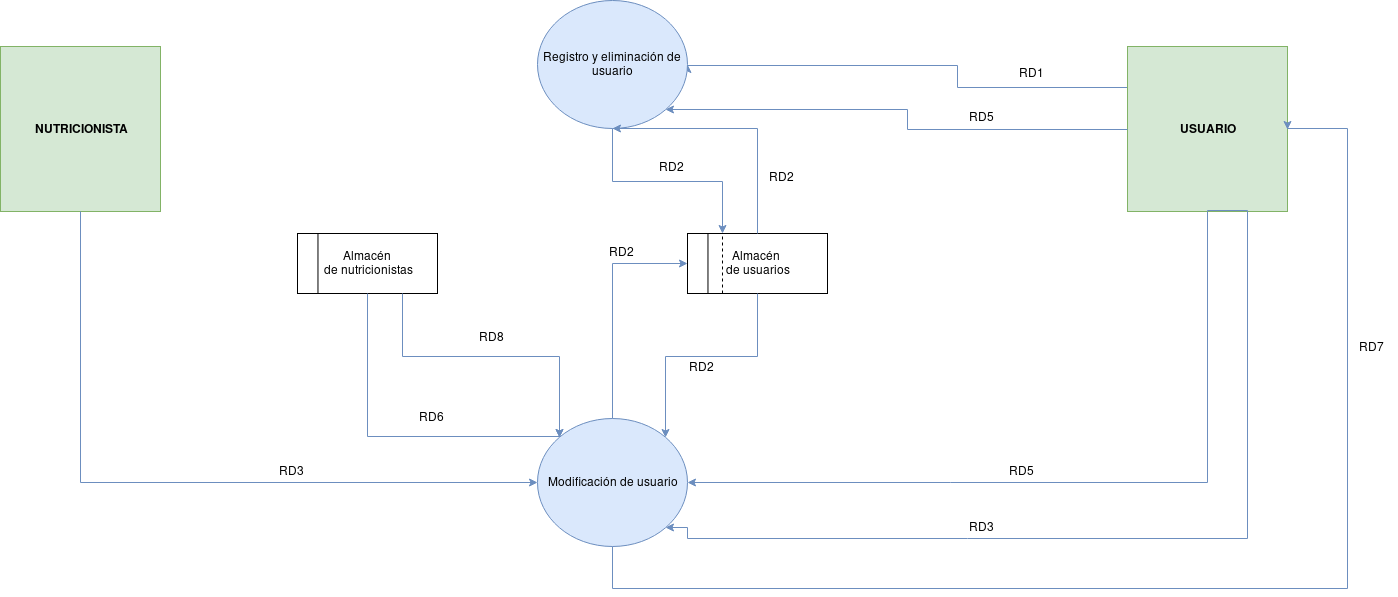
\includegraphics[scale=0.3]{Refinamiento_1_Usuarios.png}
\subsection{Refinamiento 2}
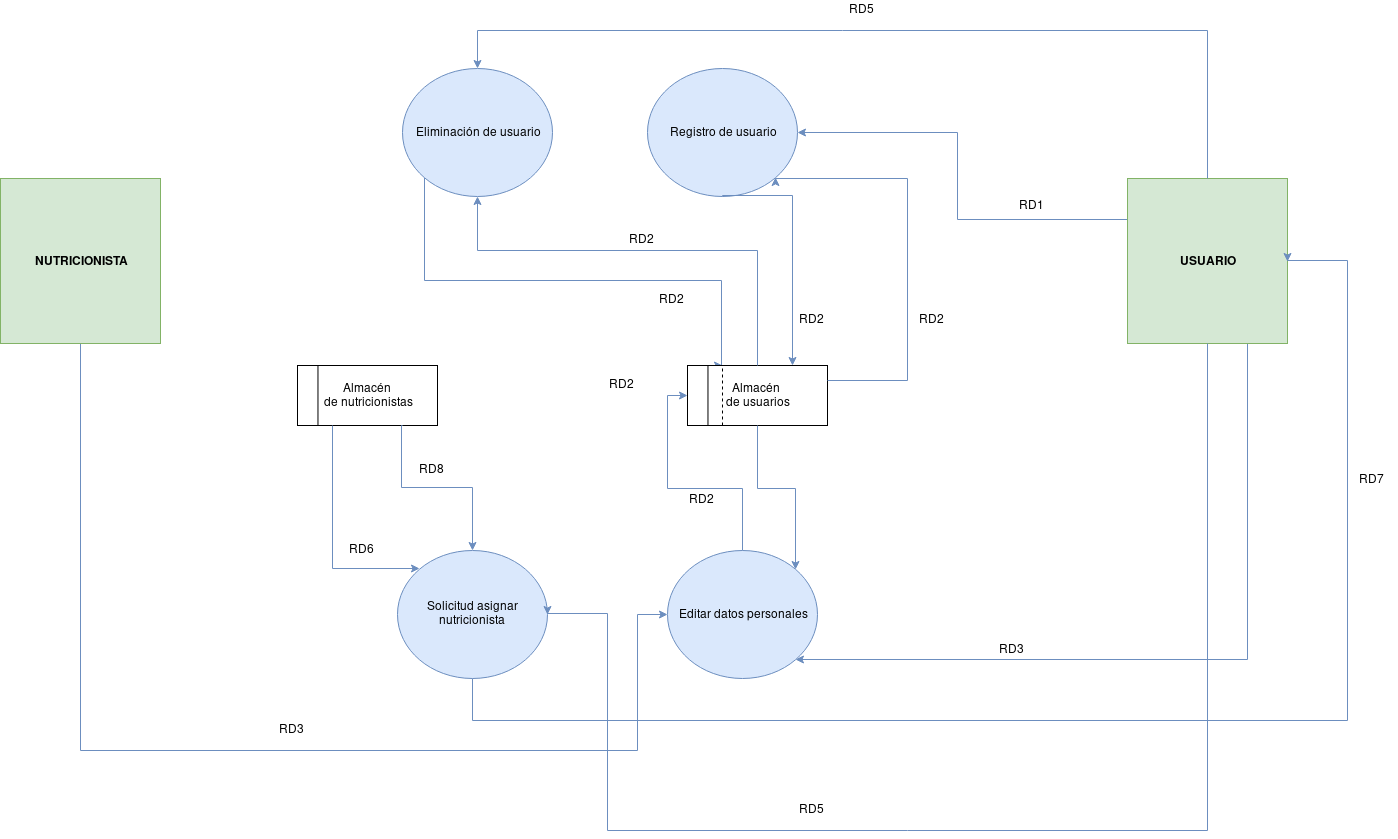
\includegraphics[scale=0.3]{Refinamiento_2_Usuarios.png}
\newpage
\subsection{Diagramas de dietas. Guillermo Bueno Vargas}
\subsection{Refinamiento 1}
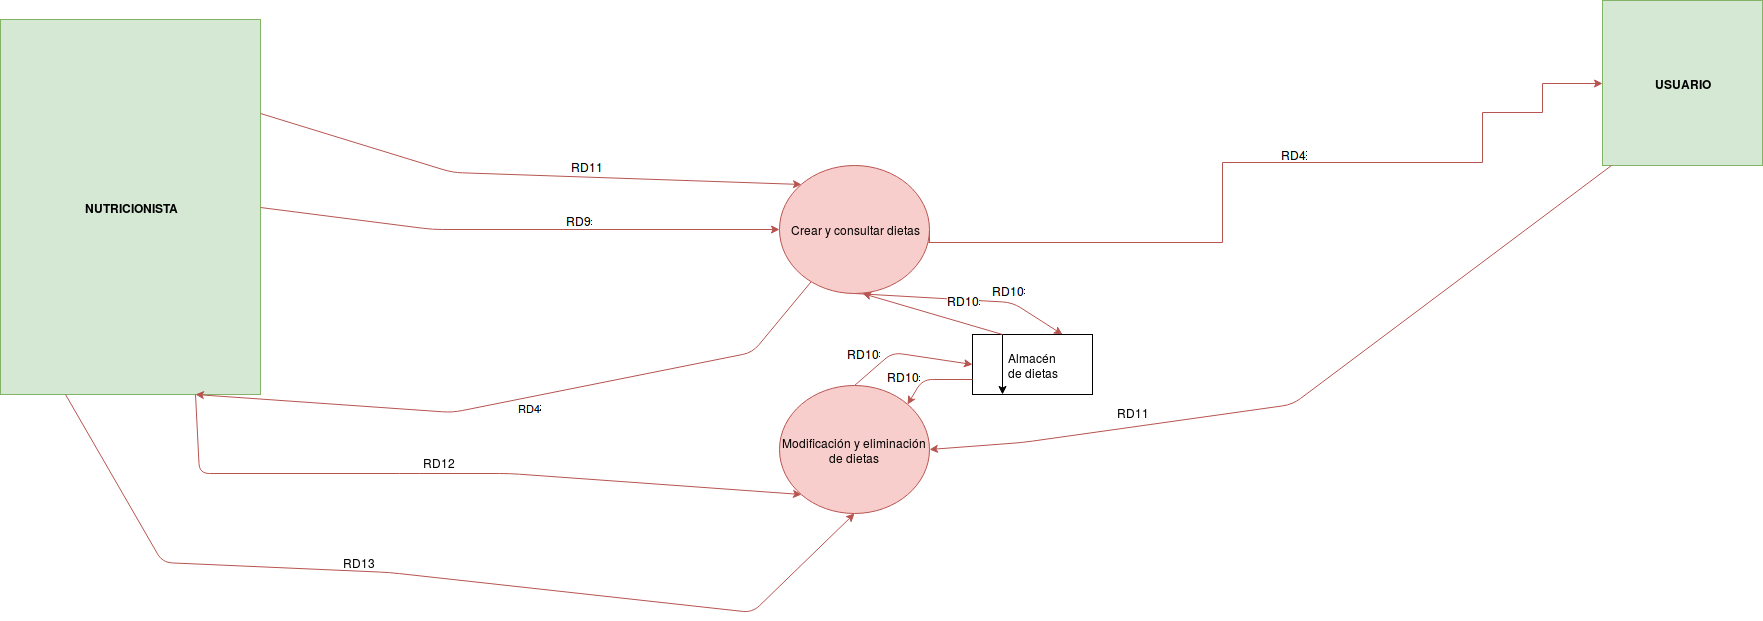
\includegraphics[scale=0.3]{Refinamiento_1_Dietas.png}
\subsection{Refinamiento 2}
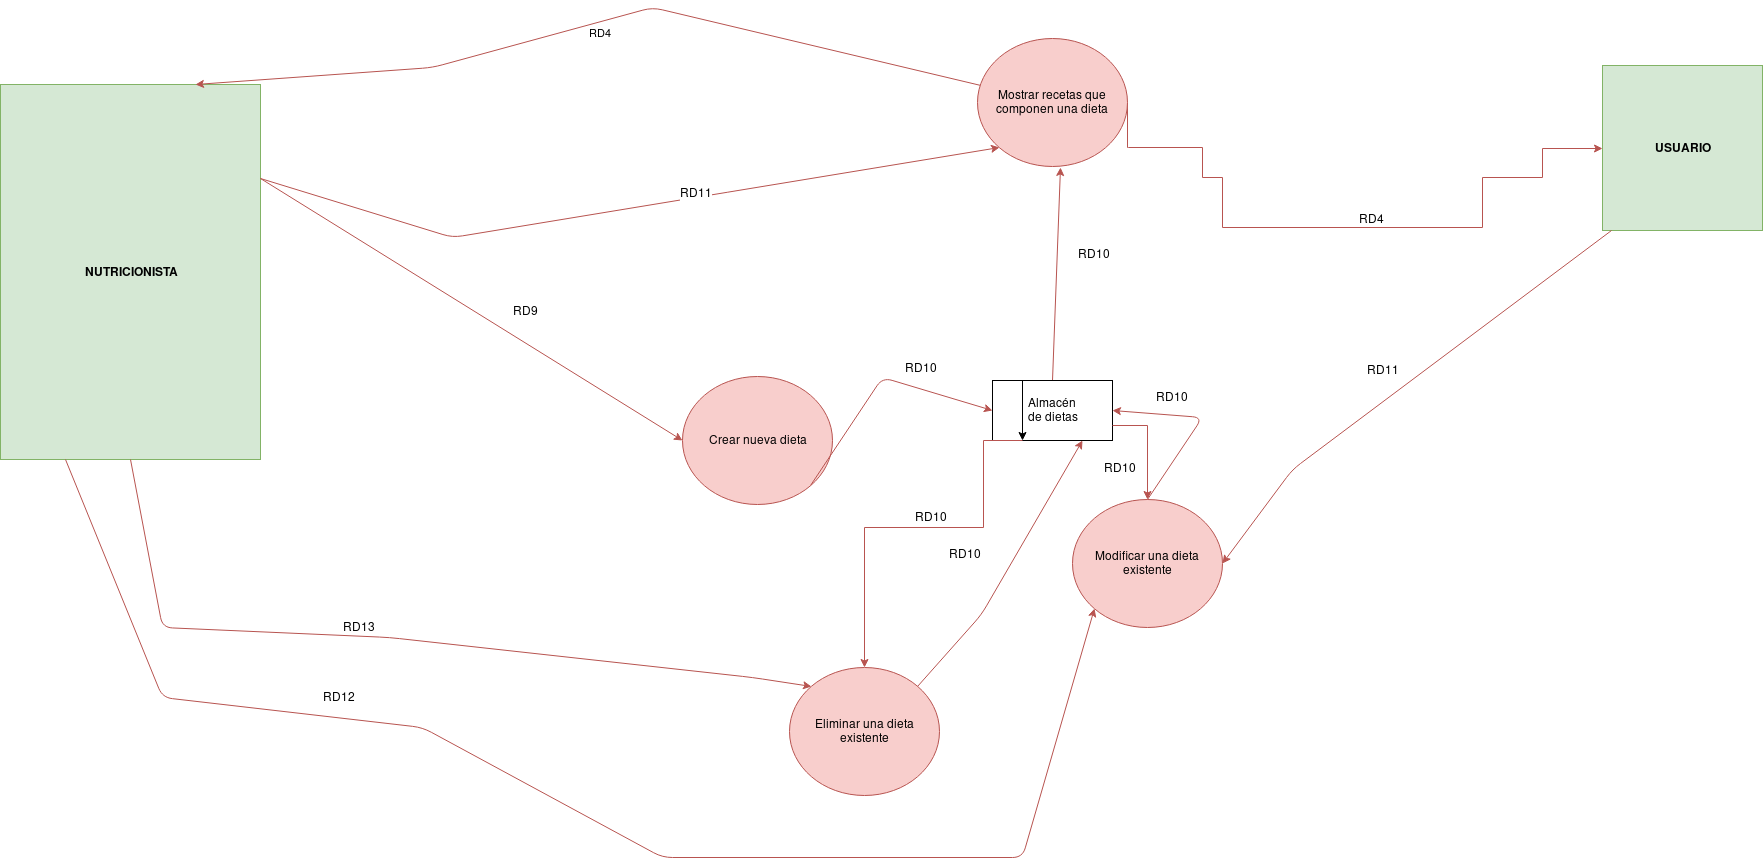
\includegraphics[scale=0.3]{Refinamiento_2_Dietas.png}
\newpage
\subsection{Diagramas de recetas. Juan Luis Sánchez}
\subsection{Refinamiento 1}
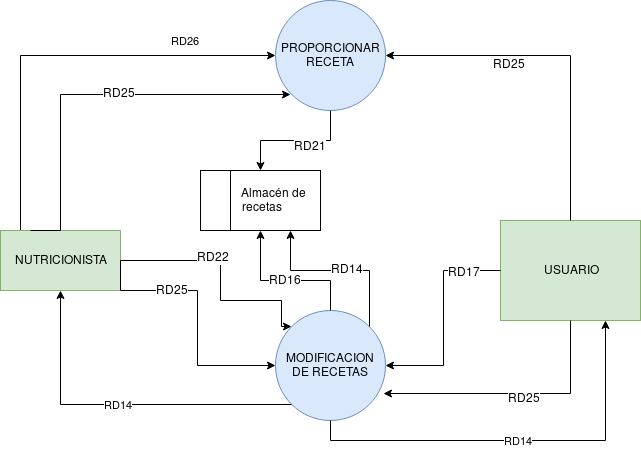
\includegraphics[scale=0.5]{Refinamiento_1_Recetas.png}
\subsection{Refinamiento 2}
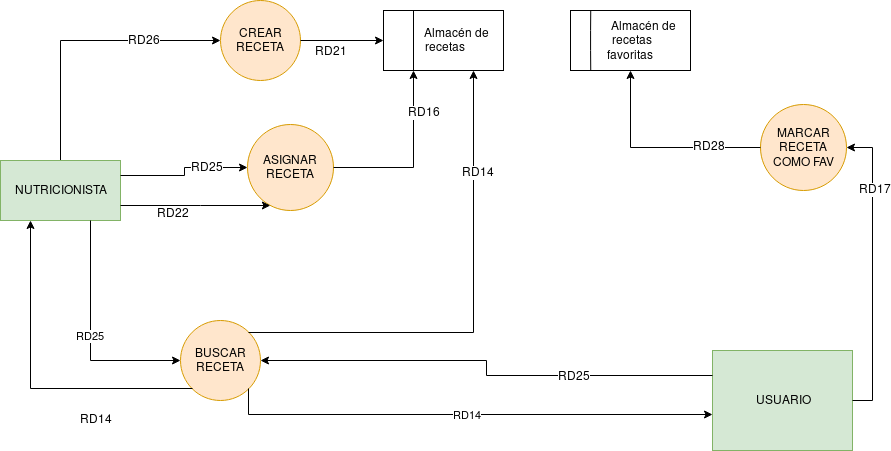
\includegraphics[scale=0.5]{Refinamiento_2_Recetas.png}
\newpage
\subsection{Diagramas de ingredientes. Arturo Cortés Sánchez}
\subsection{Refinamiento 1}
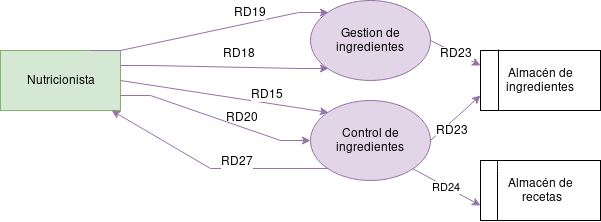
\includegraphics[scale=0.7]{Refinamineto_ingredientes.png}
\subsection{Refinamiento 2}
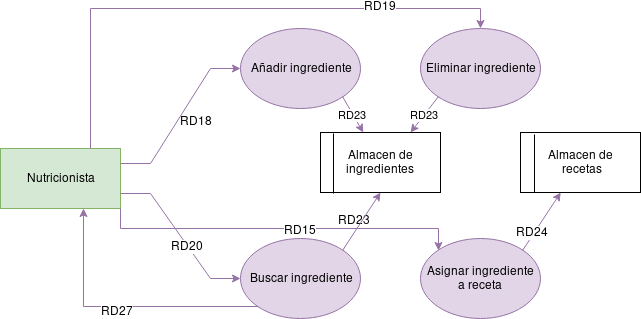
\includegraphics[scale=0.7]{Refinamiento_ingredientes_2.png}
\newpage
\subsection{Diagramas general}
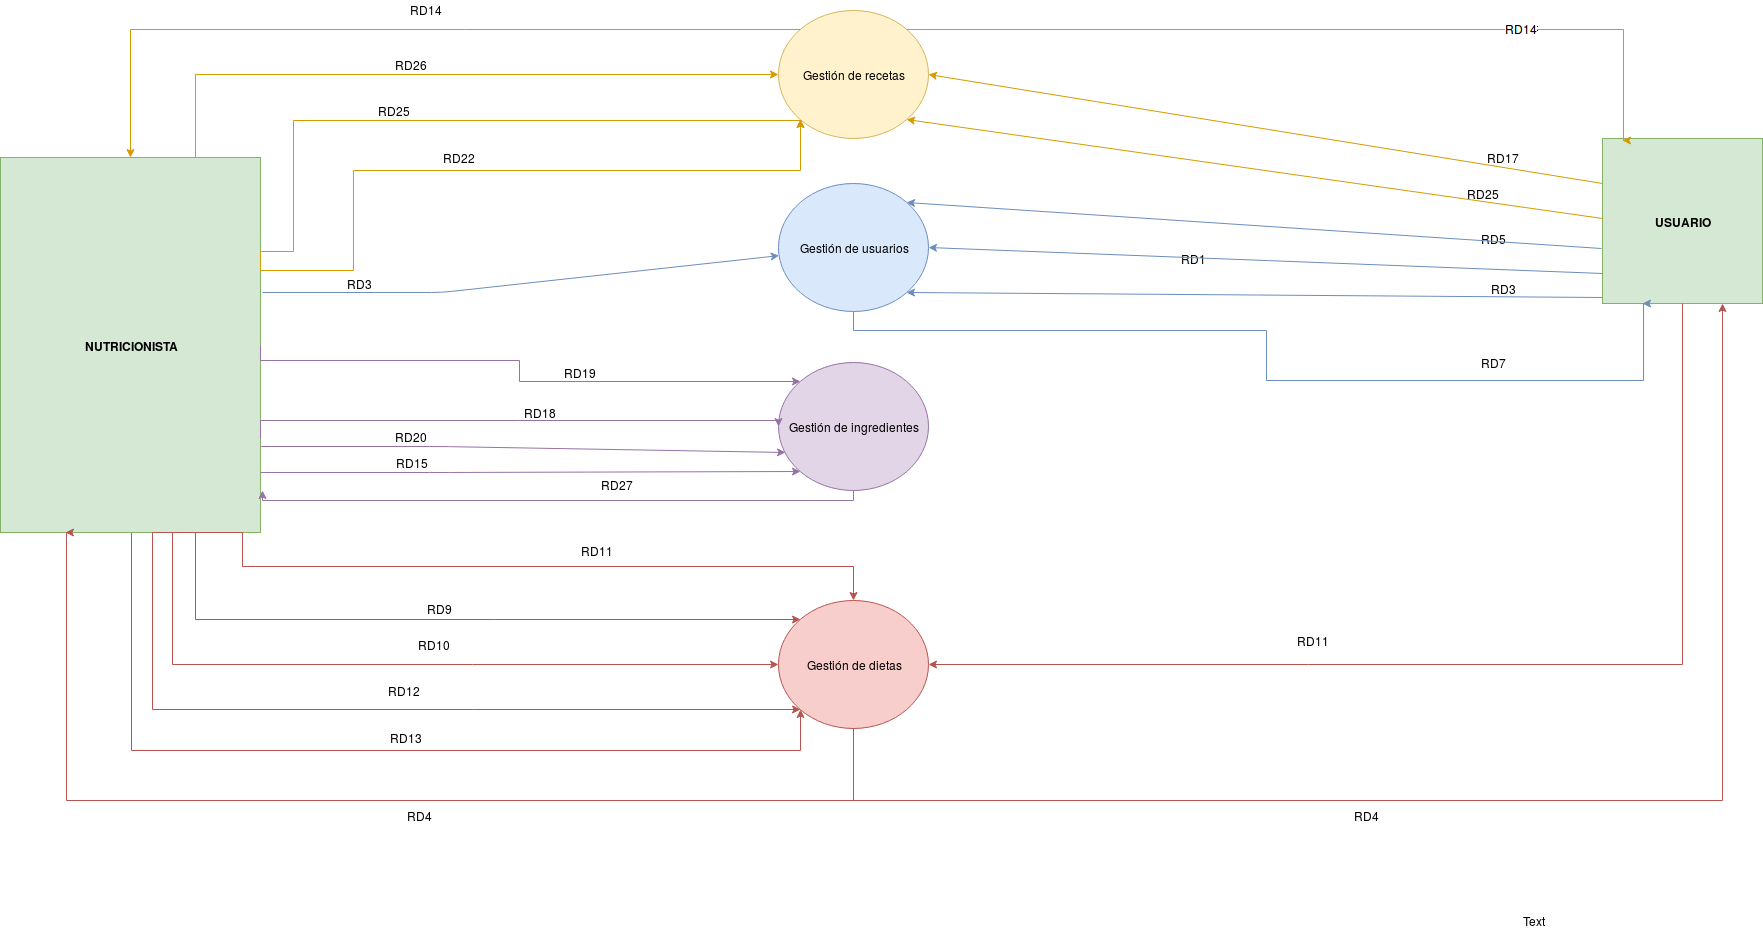
\includegraphics[scale=0.3]{Refinamiento_0.png}
\subsection{Refinamiento 1}
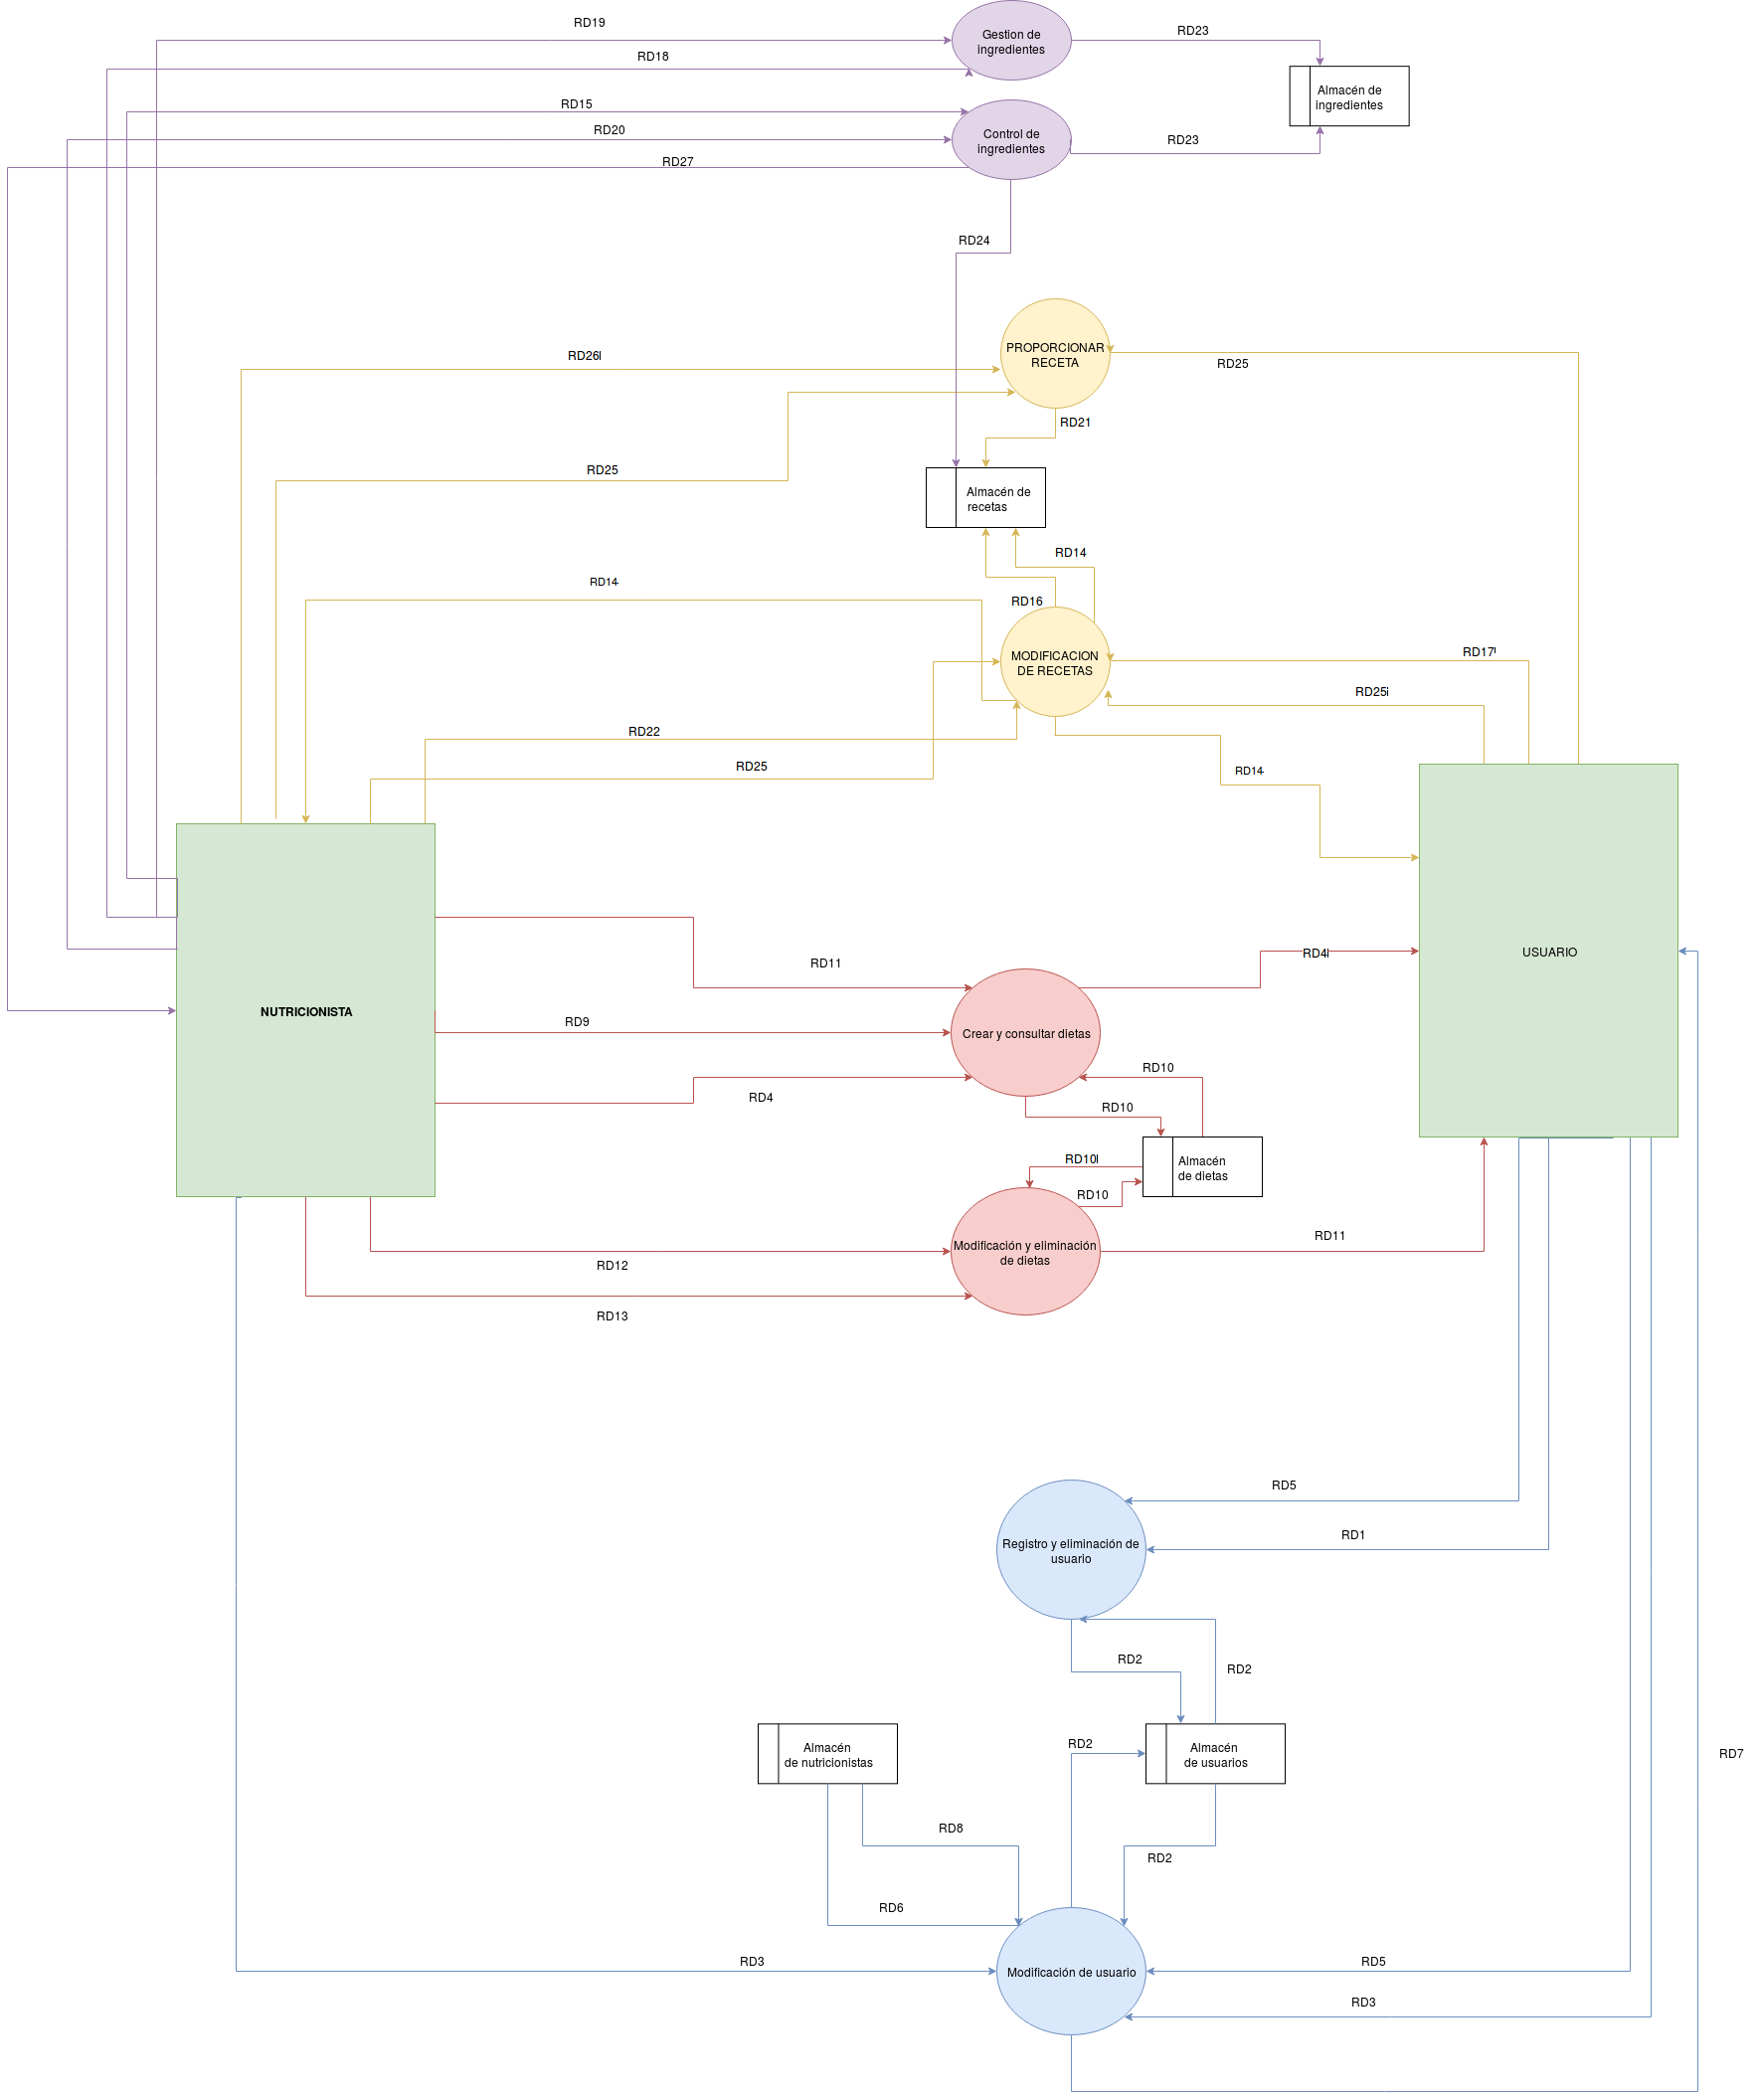
\includegraphics[scale=0.3]{Refinamiento_1.png}
\subsection{Refinamiento 2}
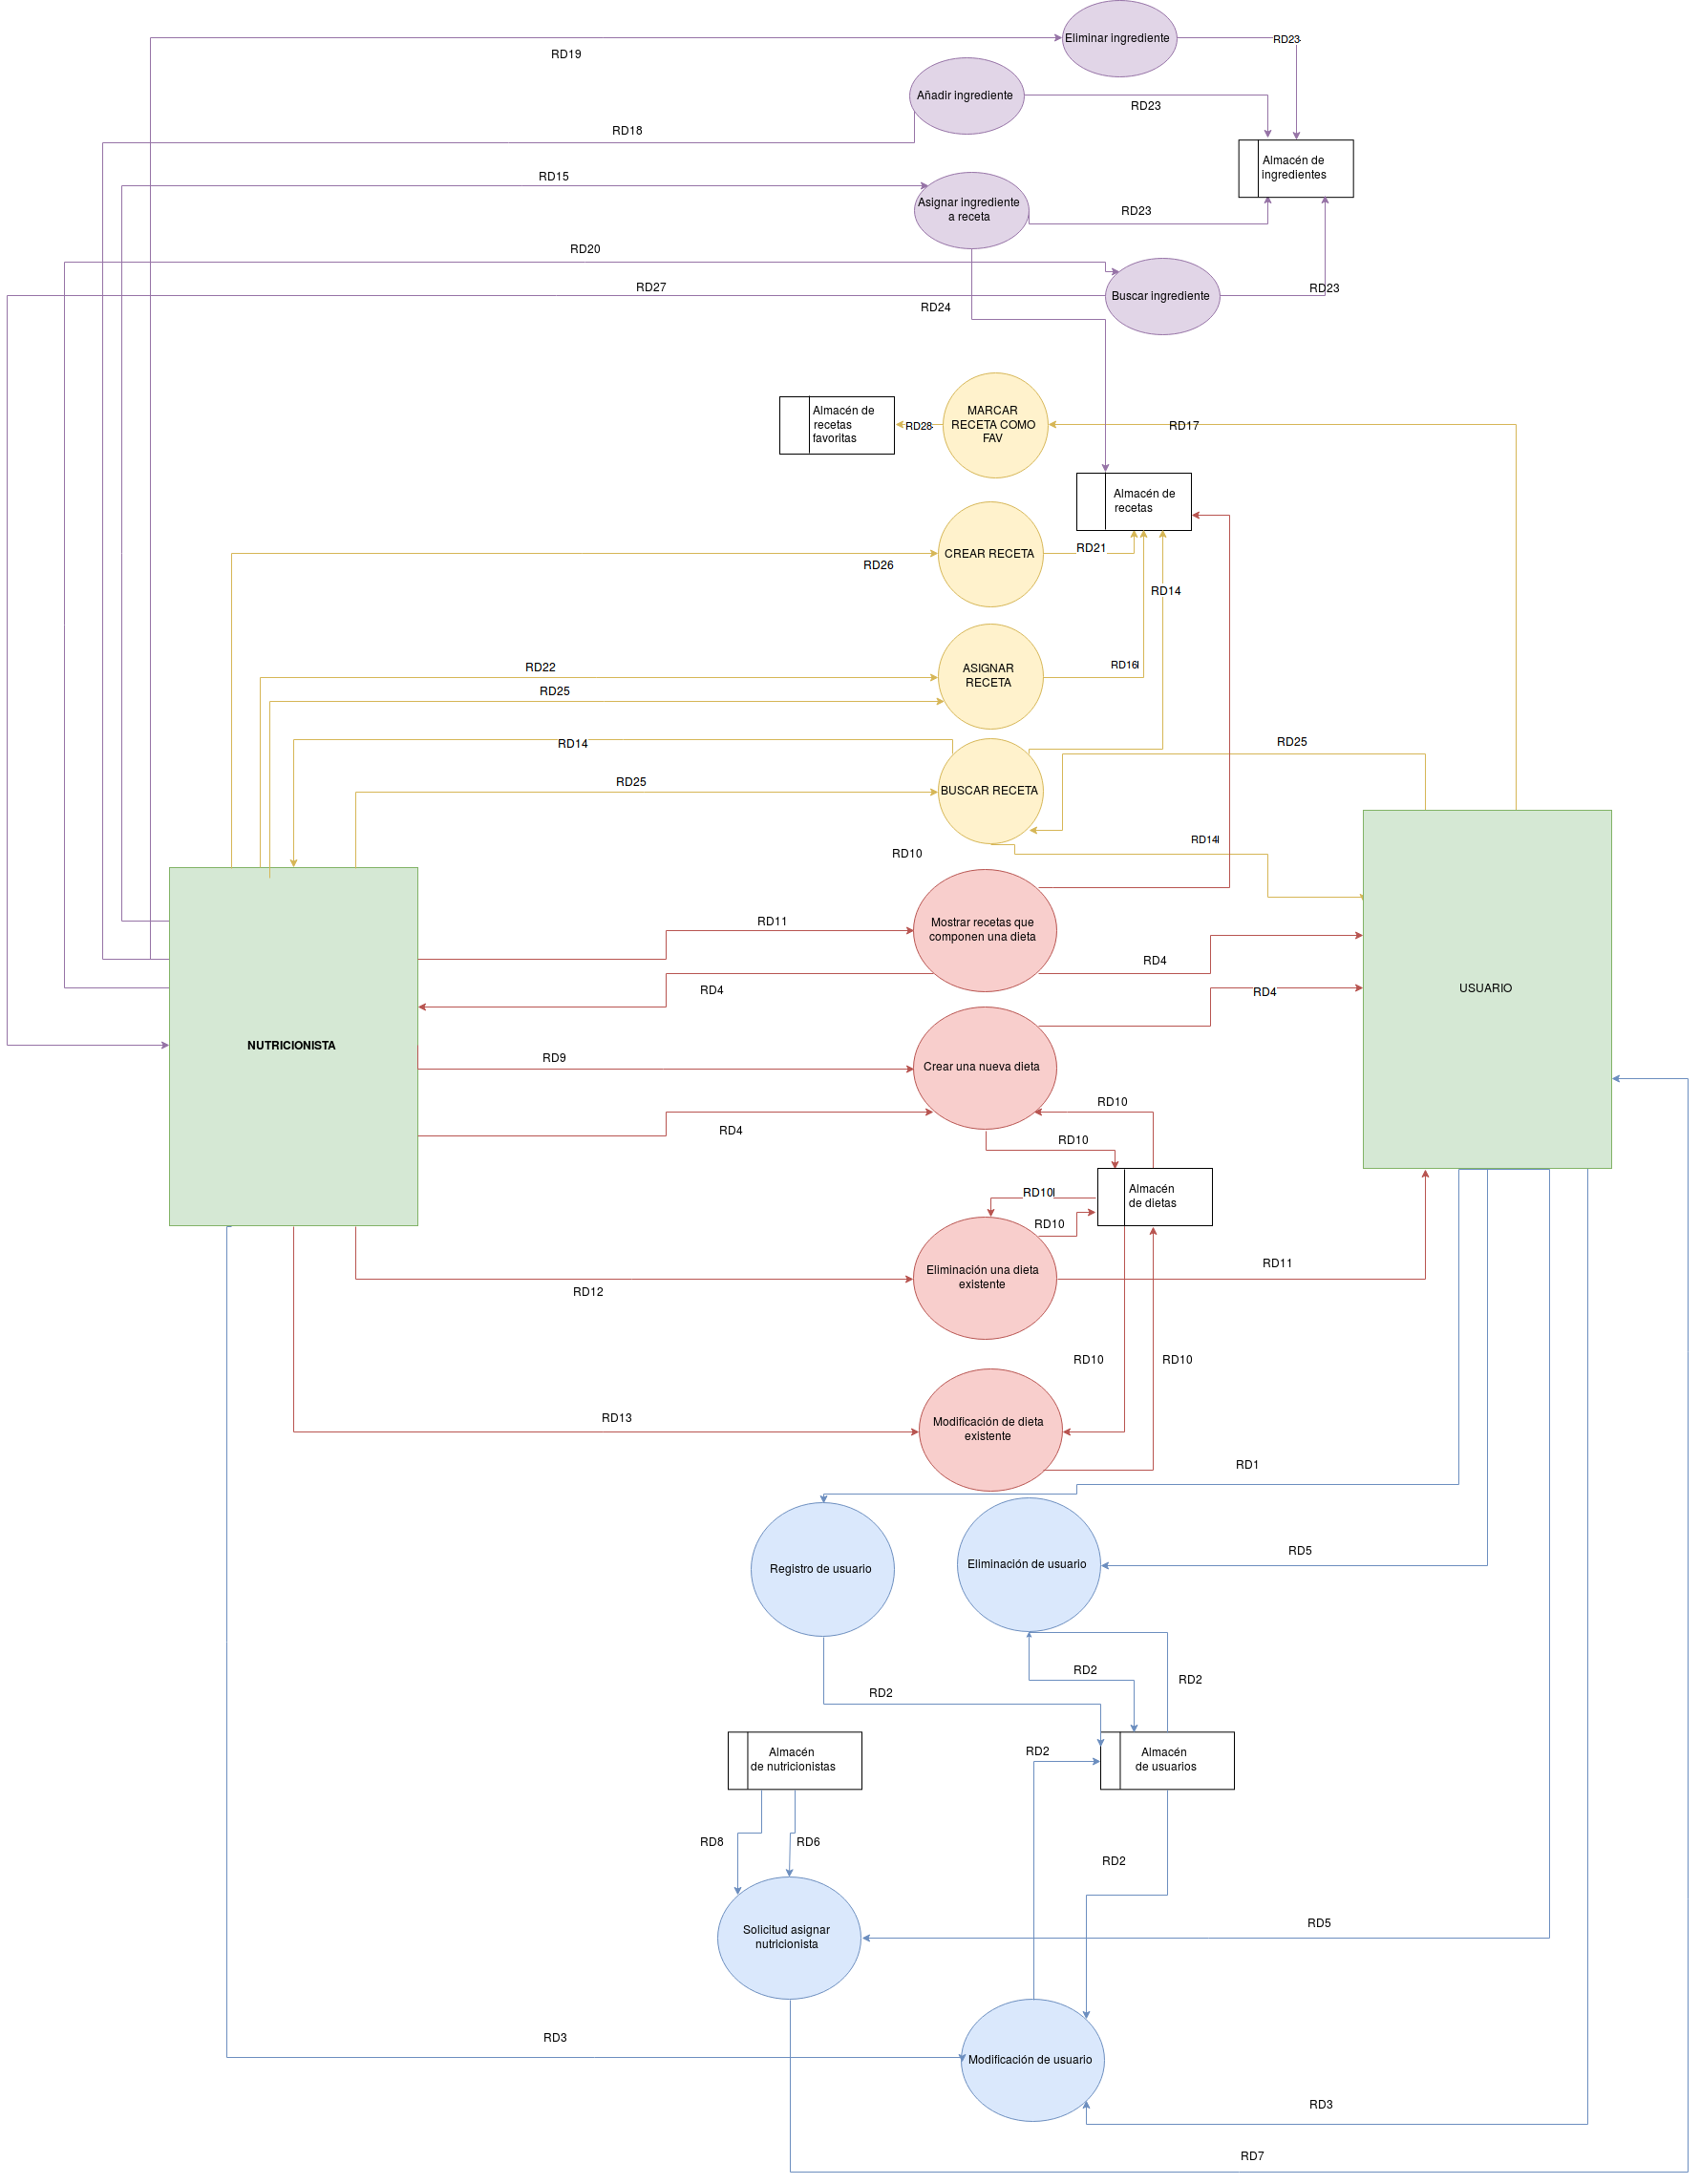
\includegraphics[scale=0.3]{Refinamiento_2.png}

\section{Diagrama Entidad-Relación}
Al no poder refinar el diagrama entidad-relación sólo se ha podido realizar un diagrama sin más.\\
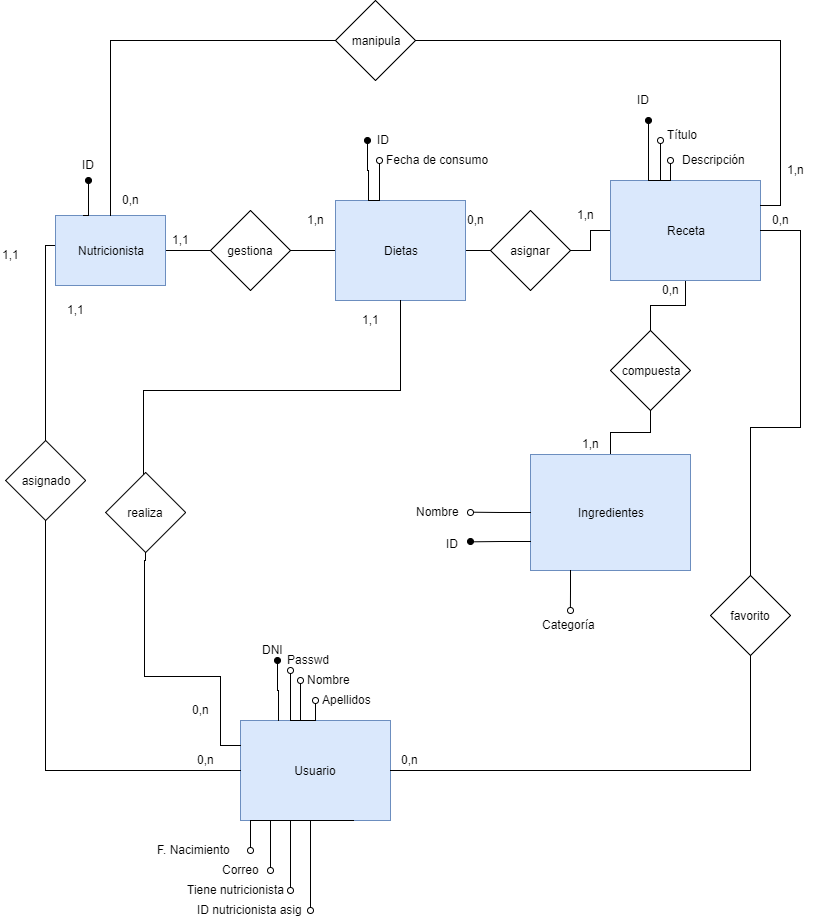
\includegraphics[scale=0.6]{entidad.png}
\newpage

\section{Diagrama Externos}
\subsection{Refinamiento 0}
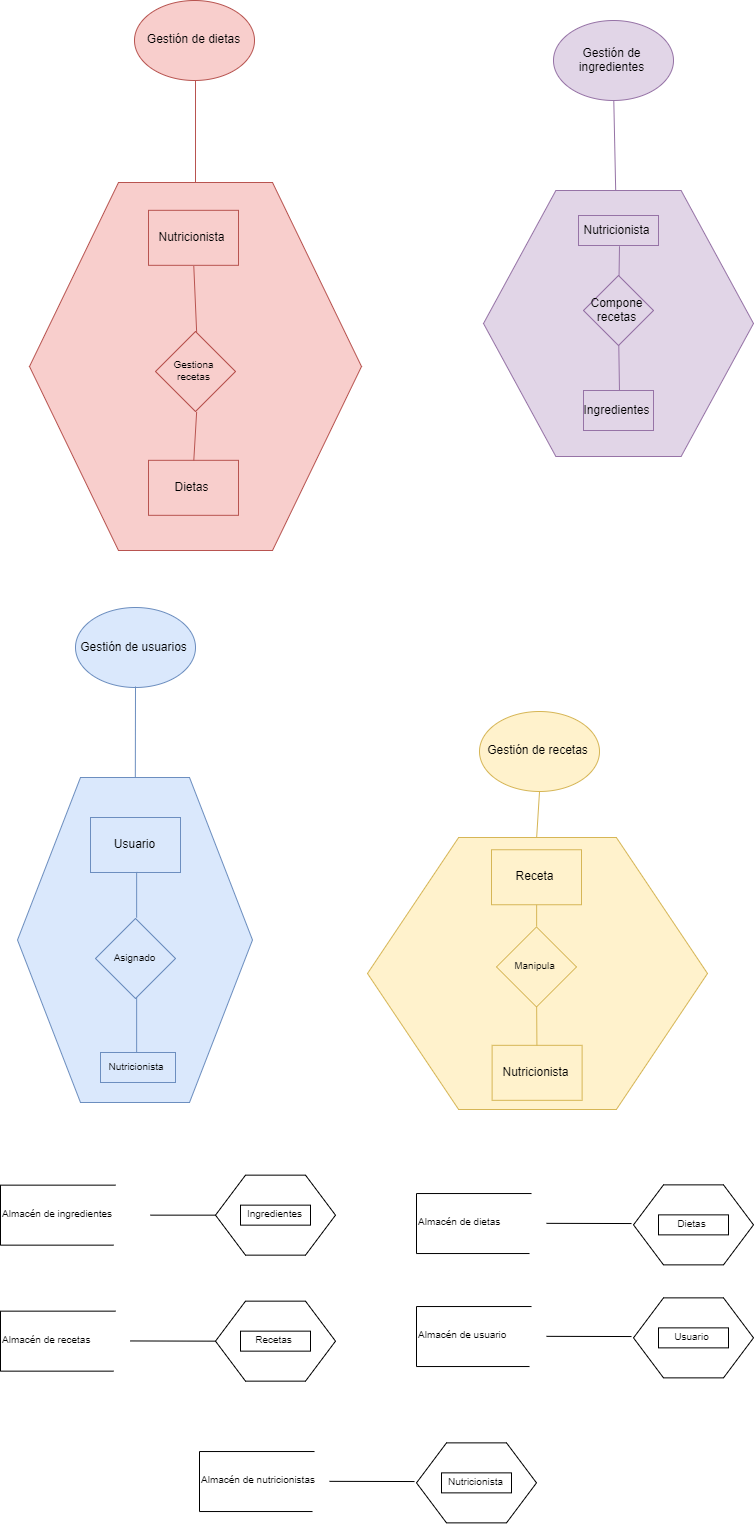
\includegraphics[scale=0.3]{externo0.png}
\subsection{Refinamiento 1}
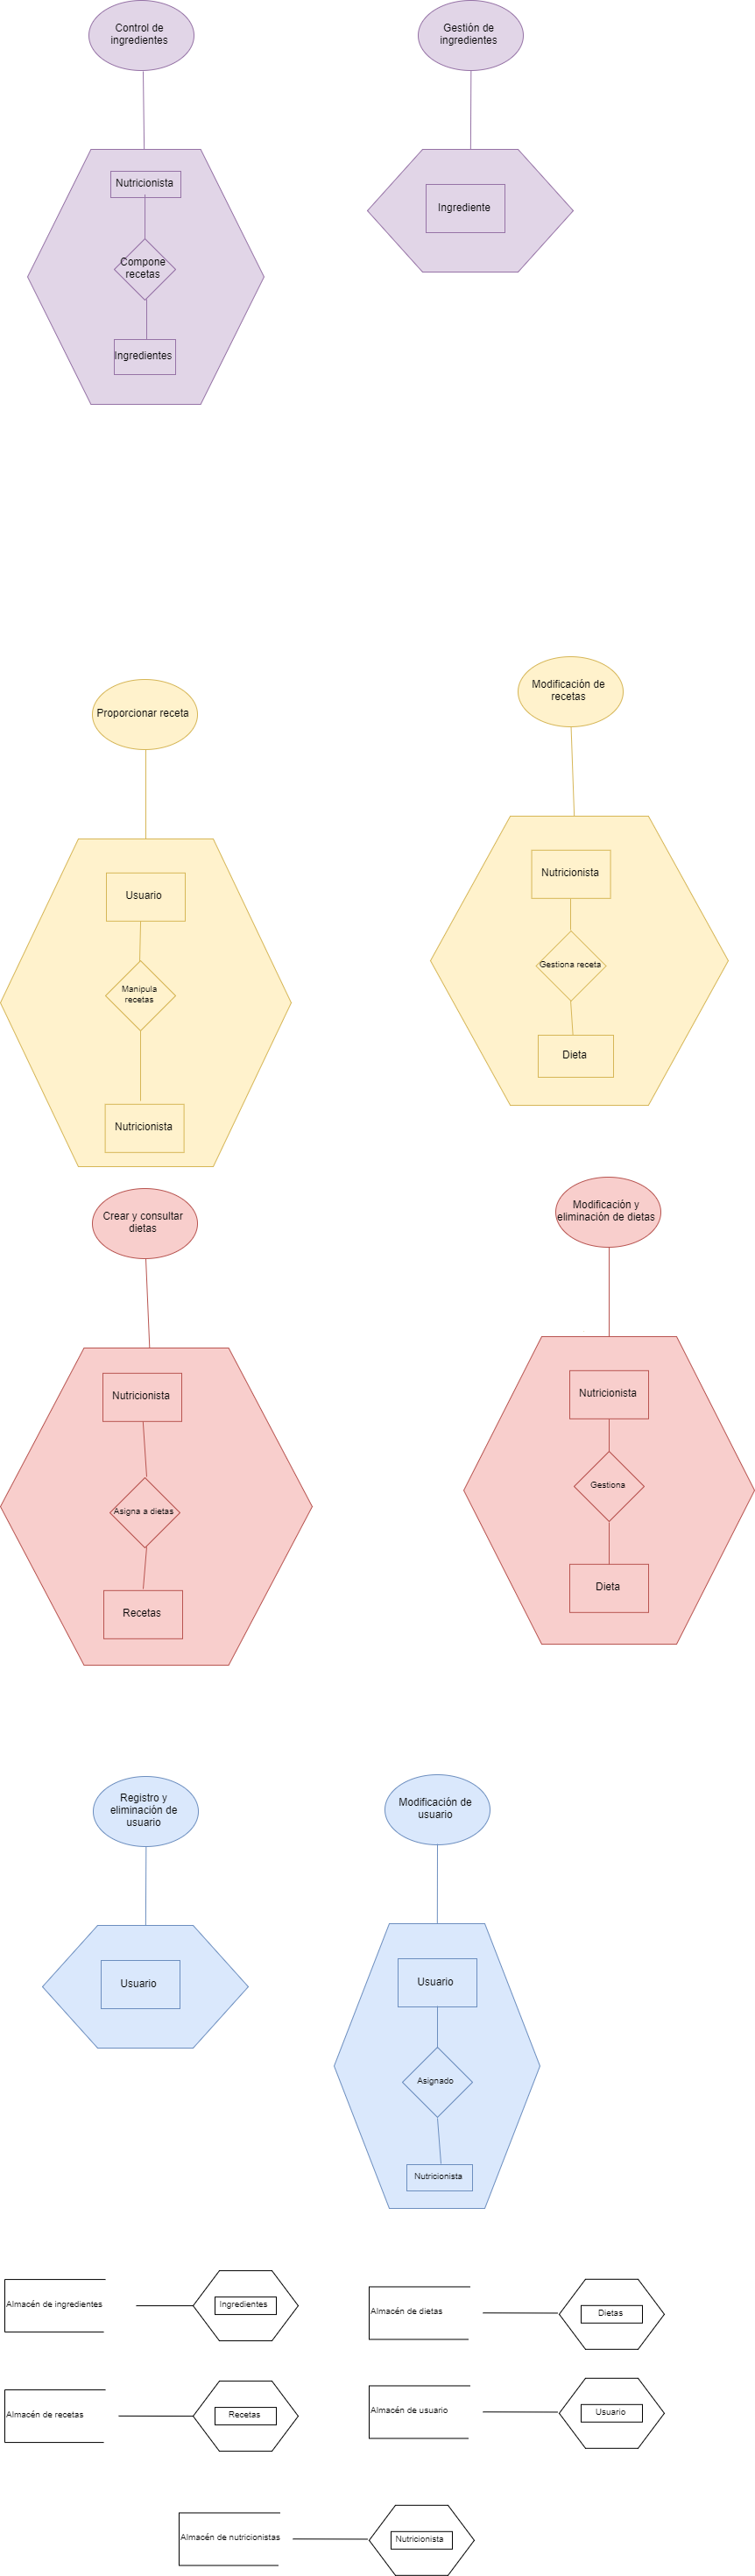
\includegraphics[scale=0.2]{externo1.png}
\subsection{Refinamiento 2}
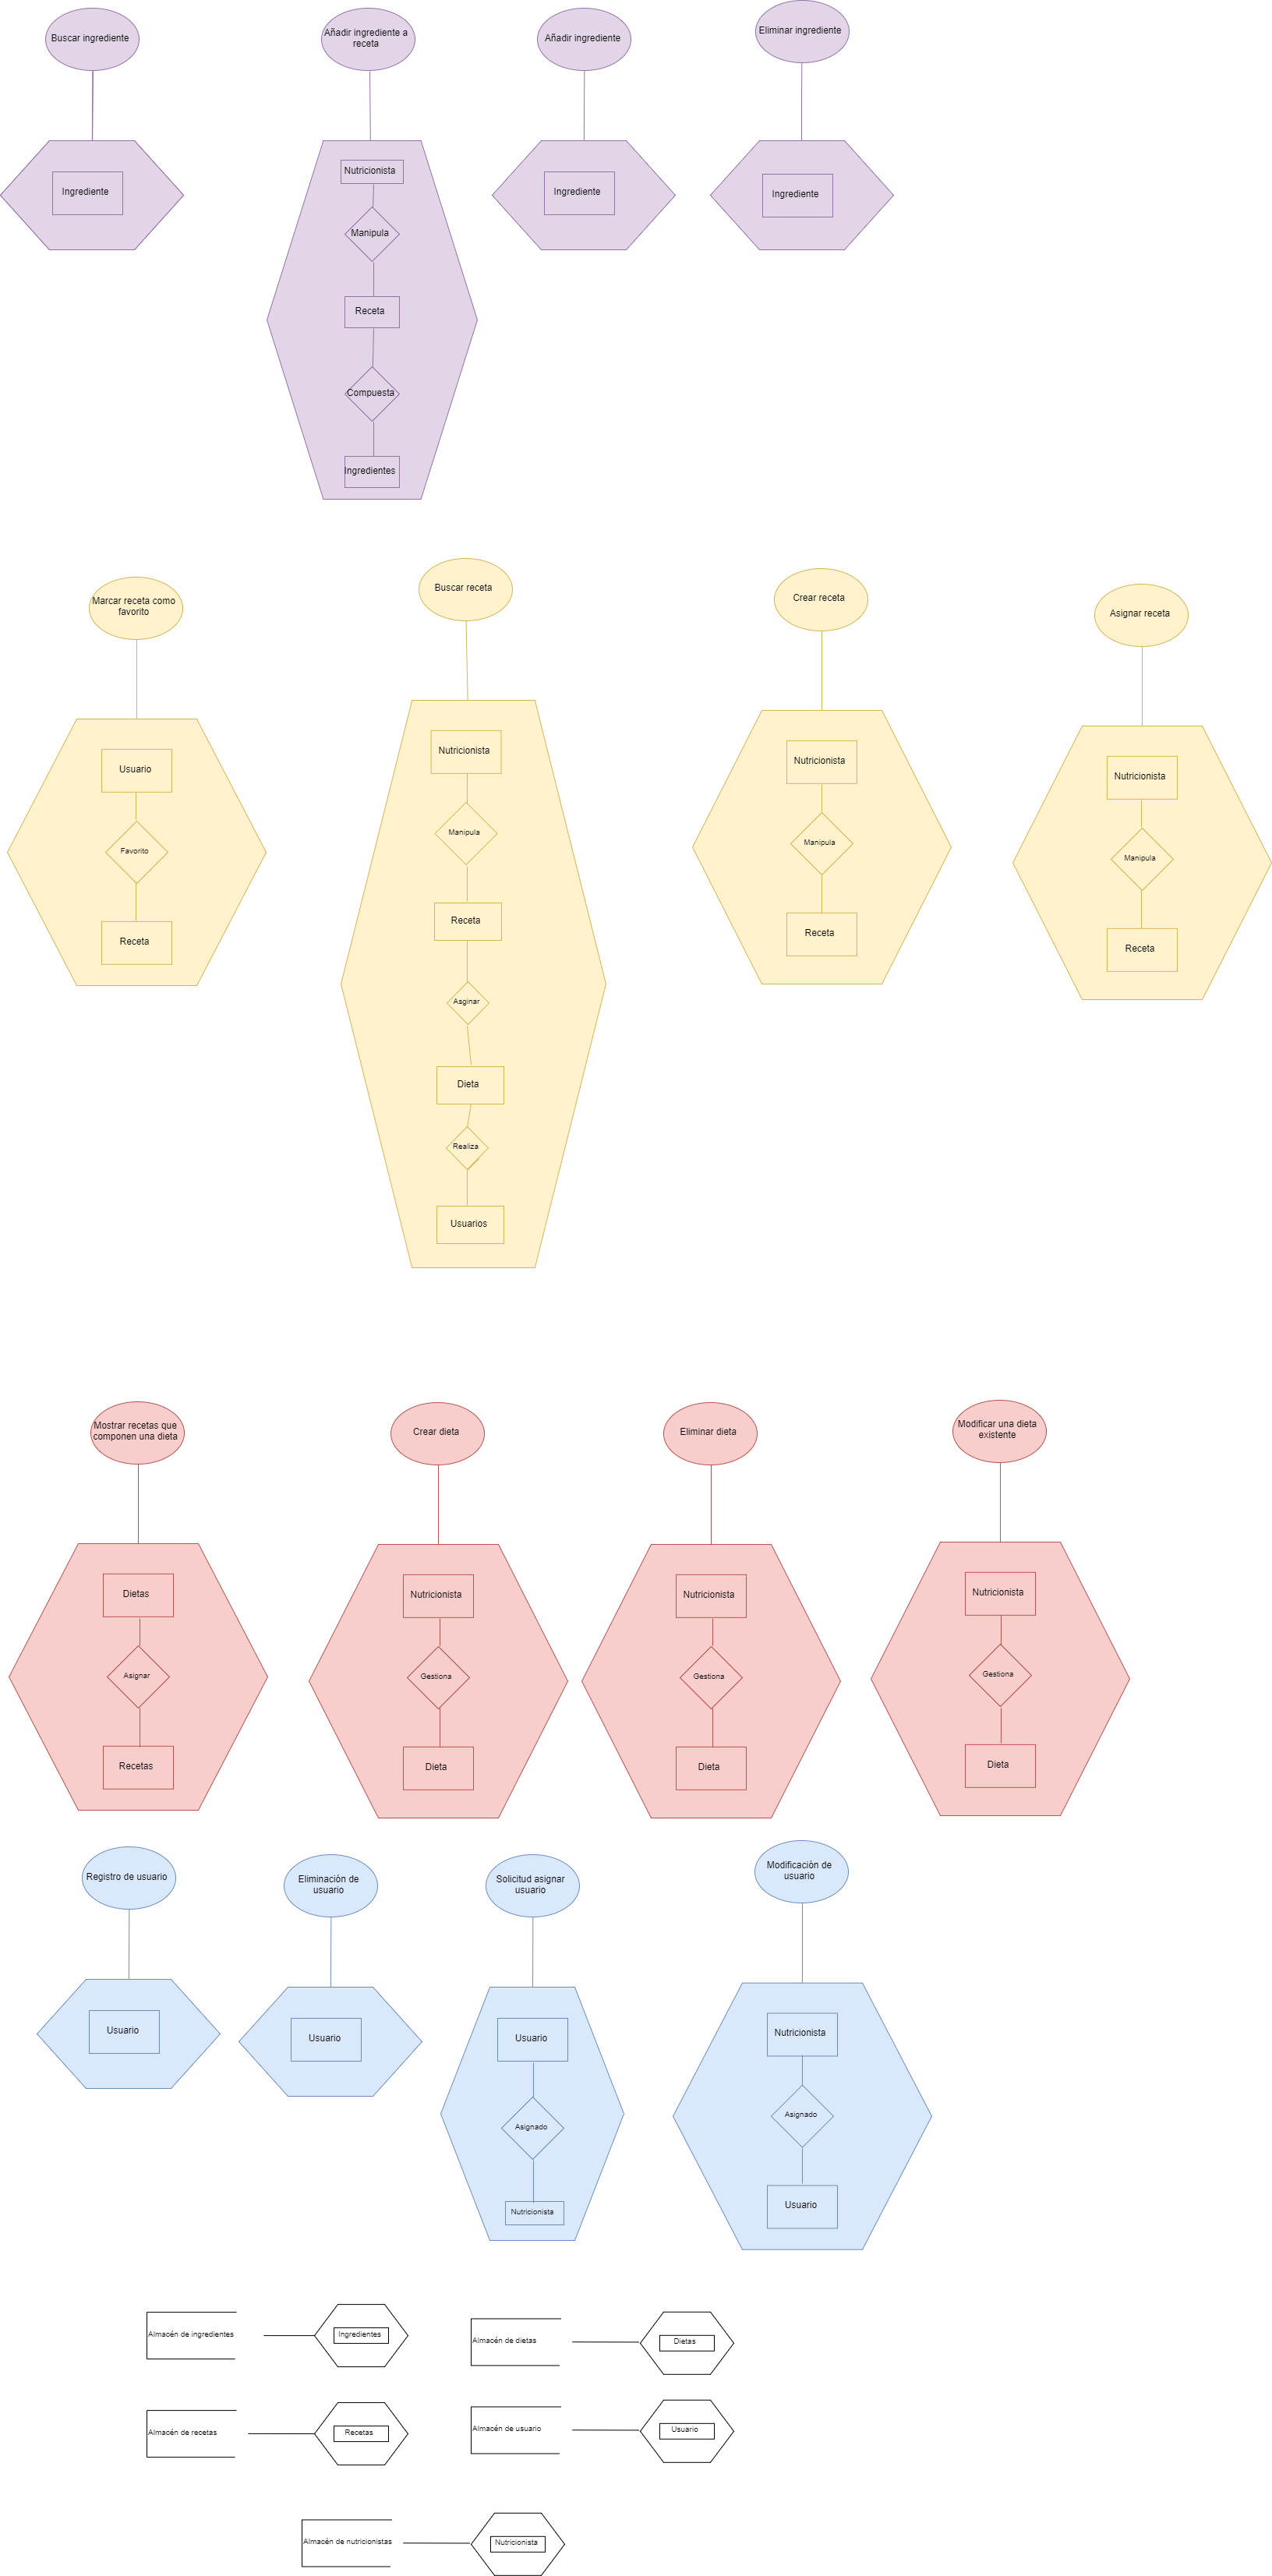
\includegraphics[scale=0.2]{externo2.png}

\section{Operaciones CRUD}
\subsection{Operación de Crear(Create)}
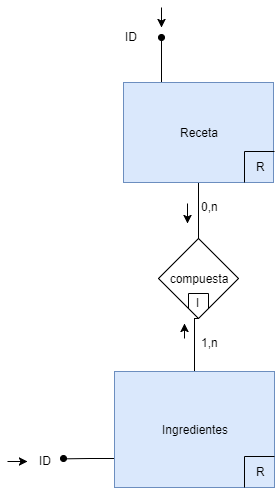
\includegraphics[scale=0.6]{Asignar.png}
\subsection{Operación de Consutar(Request)}
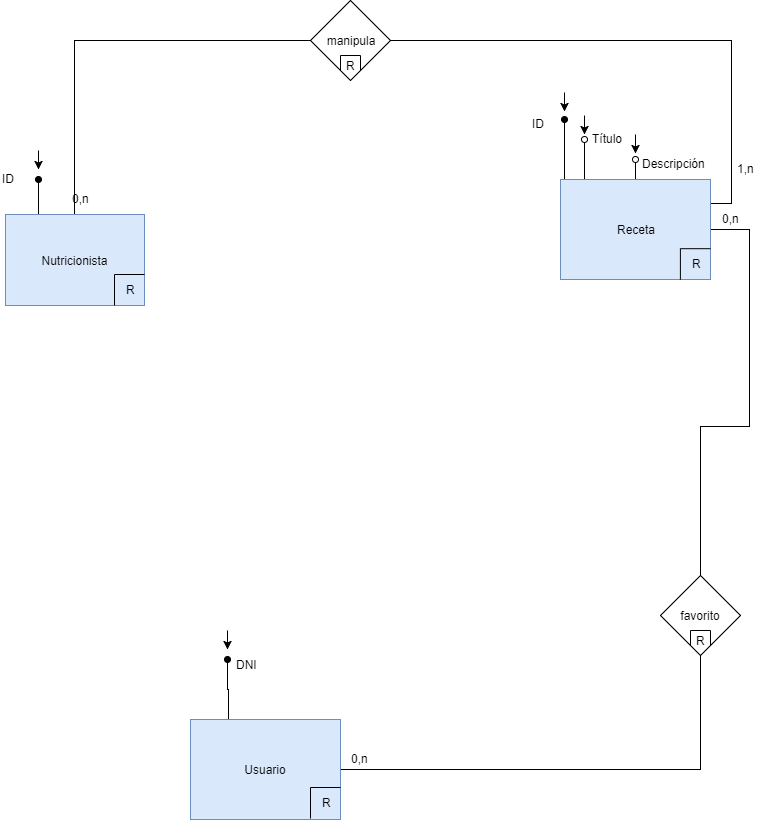
\includegraphics[scale=0.3]{Buscar.png}
\subsection{Operación de Actualizar(Update)}
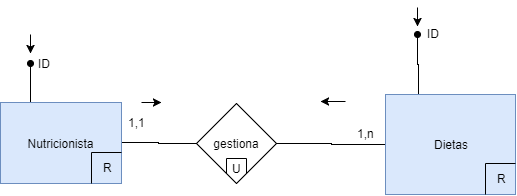
\includegraphics[scale=0.6]{Modificar.png}
\subsection{Operación de Eliminar(Delete)}
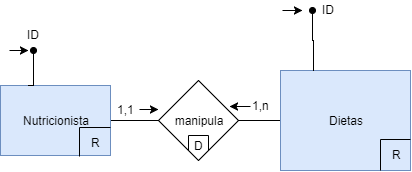
\includegraphics[scale=0.6]{Borrar.png}

\section{Paso a tabla del E/R}
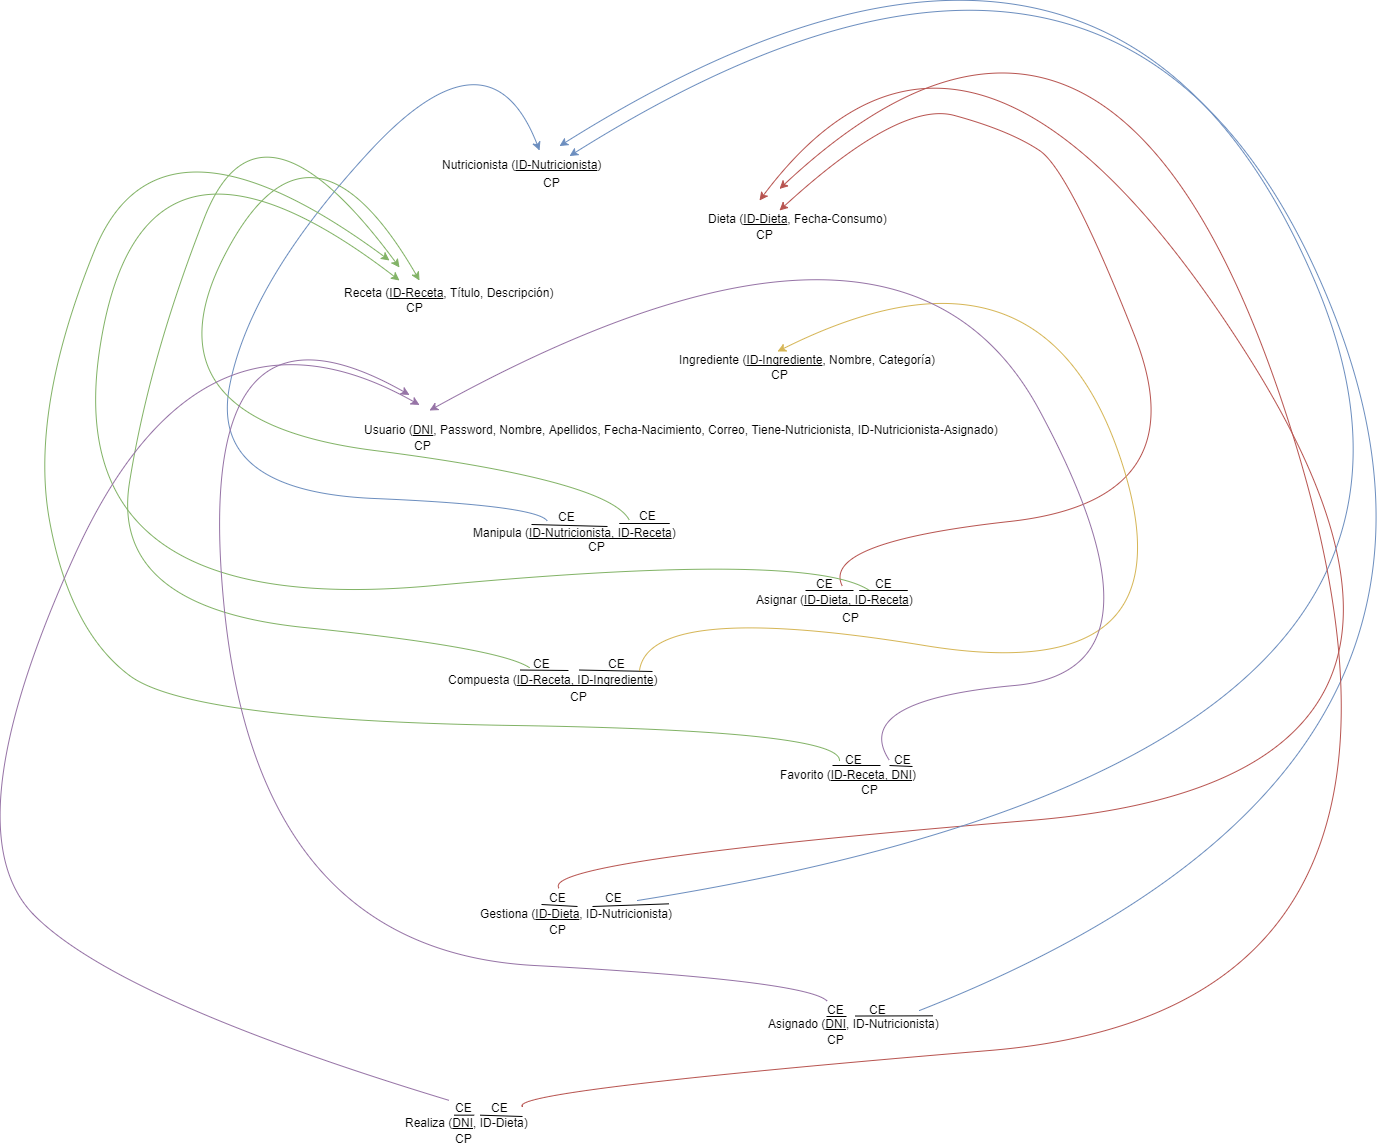
\includegraphics[scale=0.35]{Tabla.png}
\newpage

\section{Implementación}
Para la implementación se ha usado NetBeans, Java 8 y MySQL Workbench.


\section{Sentencias SQL}

\subsection{Asignar}
\begin{lstlisting}[language=sql]
-- MySQL dump 10.13  Distrib 5.7.20, for Linux (x86_64)
--
-- Host: localhost    Database: ohmydiet!
-- ------------------------------------------------------
-- Server version	5.7.20-0ubuntu0.16.04.1

/*!40101 SET @OLD_CHARACTER_SET_CLIENT=@@CHARACTER_SET_CLIENT */;
/*!40101 SET @OLD_CHARACTER_SET_RESULTS=@@CHARACTER_SET_RESULTS */;
/*!40101 SET @OLD_COLLATION_CONNECTION=@@COLLATION_CONNECTION */;
/*!40101 SET NAMES utf8 */;
/*!40103 SET @OLD_TIME_ZONE=@@TIME_ZONE */;
/*!40103 SET TIME_ZONE='+00:00' */;
/*!40014 SET @OLD_UNIQUE_CHECKS=@@UNIQUE_CHECKS, UNIQUE_CHECKS=0 */;
/*!40014 SET @OLD_FOREIGN_KEY_CHECKS=@@FOREIGN_KEY_CHECKS, FOREIGN_KEY_CHECKS=0 */;
/*!40101 SET @OLD_SQL_MODE=@@SQL_MODE, SQL_MODE='NO_AUTO_VALUE_ON_ZERO' */;
/*!40111 SET @OLD_SQL_NOTES=@@SQL_NOTES, SQL_NOTES=0 */;

--
-- Table structure for table `asignado`
--

DROP TABLE IF EXISTS `asignado`;
/*!40101 SET @saved_cs_client     = @@character_set_client */;
/*!40101 SET character_set_client = utf8 */;
CREATE TABLE `asignado` (
`DNI` varchar(50) NOT NULL,
`id_nutricionista` int(10) unsigned NOT NULL,
PRIMARY KEY (`DNI`),
KEY `FK__nutricionist3` (`id_nutricionista`),
CONSTRAINT `FK__nutricionist3` FOREIGN KEY (`id_nutricionista`) REFERENCES `nutricionista` (`id_nutricionista`),
CONSTRAINT `FK__usuario3` FOREIGN KEY (`DNI`) REFERENCES `usuario` (`DNI`)
) ENGINE=InnoDB DEFAULT CHARSET=latin1;
/*!40101 SET character_set_client = @saved_cs_client */;

--
-- Dumping data for table `asignado`
--

LOCK TABLES `asignado` WRITE;
/*!40000 ALTER TABLE `asignado` DISABLE KEYS */;
/*!40000 ALTER TABLE `asignado` ENABLE KEYS */;
UNLOCK TABLES;
/*!40103 SET TIME_ZONE=@OLD_TIME_ZONE */;

/*!40101 SET SQL_MODE=@OLD_SQL_MODE */;
/*!40014 SET FOREIGN_KEY_CHECKS=@OLD_FOREIGN_KEY_CHECKS */;
/*!40014 SET UNIQUE_CHECKS=@OLD_UNIQUE_CHECKS */;
/*!40101 SET CHARACTER_SET_CLIENT=@OLD_CHARACTER_SET_CLIENT */;
/*!40101 SET CHARACTER_SET_RESULTS=@OLD_CHARACTER_SET_RESULTS */;
/*!40101 SET COLLATION_CONNECTION=@OLD_COLLATION_CONNECTION */;
/*!40111 SET SQL_NOTES=@OLD_SQL_NOTES */;

-- Dump completed on 2018-01-20 20:55:17

\end{lstlisting}
\subsection{Compuesta}
\begin{lstlisting}[language=sql]
-- MySQL dump 10.13  Distrib 5.7.20, for Linux (x86_64)
--
-- Host: localhost    Database: ohmydiet!
-- ------------------------------------------------------
-- Server version	5.7.20-0ubuntu0.16.04.1

/*!40101 SET @OLD_CHARACTER_SET_CLIENT=@@CHARACTER_SET_CLIENT */;
/*!40101 SET @OLD_CHARACTER_SET_RESULTS=@@CHARACTER_SET_RESULTS */;
/*!40101 SET @OLD_COLLATION_CONNECTION=@@COLLATION_CONNECTION */;
/*!40101 SET NAMES utf8 */;
/*!40103 SET @OLD_TIME_ZONE=@@TIME_ZONE */;
/*!40103 SET TIME_ZONE='+00:00' */;
/*!40014 SET @OLD_UNIQUE_CHECKS=@@UNIQUE_CHECKS, UNIQUE_CHECKS=0 */;
/*!40014 SET @OLD_FOREIGN_KEY_CHECKS=@@FOREIGN_KEY_CHECKS, FOREIGN_KEY_CHECKS=0 */;
/*!40101 SET @OLD_SQL_MODE=@@SQL_MODE, SQL_MODE='NO_AUTO_VALUE_ON_ZERO' */;
/*!40111 SET @OLD_SQL_NOTES=@@SQL_NOTES, SQL_NOTES=0 */;

--
-- Table structure for table `asignar`
--

DROP TABLE IF EXISTS `asignar`;
/*!40101 SET @saved_cs_client     = @@character_set_client */;
/*!40101 SET character_set_client = utf8 */;
CREATE TABLE `asignar` (
`id_dieta` int(10) unsigned NOT NULL,
`id_receta` int(10) unsigned NOT NULL,
PRIMARY KEY (`id_dieta`,`id_receta`),
KEY `FK_asignar_receta` (`id_receta`),
CONSTRAINT `FK_asignar_dieta` FOREIGN KEY (`id_dieta`) REFERENCES `dieta` (`id_dieta`),
CONSTRAINT `FK_asignar_receta` FOREIGN KEY (`id_receta`) REFERENCES `receta` (`id_receta`)
) ENGINE=InnoDB DEFAULT CHARSET=latin1;
/*!40101 SET character_set_client = @saved_cs_client */;

--
-- Dumping data for table `asignar`
--

LOCK TABLES `asignar` WRITE;
/*!40000 ALTER TABLE `asignar` DISABLE KEYS */;
INSERT INTO `asignar` VALUES (0,1),(0,2),(0,4),(0,6);
/*!40000 ALTER TABLE `asignar` ENABLE KEYS */;
UNLOCK TABLES;
/*!40103 SET TIME_ZONE=@OLD_TIME_ZONE */;

/*!40101 SET SQL_MODE=@OLD_SQL_MODE */;
/*!40014 SET FOREIGN_KEY_CHECKS=@OLD_FOREIGN_KEY_CHECKS */;
/*!40014 SET UNIQUE_CHECKS=@OLD_UNIQUE_CHECKS */;
/*!40101 SET CHARACTER_SET_CLIENT=@OLD_CHARACTER_SET_CLIENT */;
/*!40101 SET CHARACTER_SET_RESULTS=@OLD_CHARACTER_SET_RESULTS */;
/*!40101 SET COLLATION_CONNECTION=@OLD_COLLATION_CONNECTION */;
/*!40111 SET SQL_NOTES=@OLD_SQL_NOTES */;

-- Dump completed on 2018-01-20 20:55:17

\end{lstlisting}
\subsection{Dieta}
\begin{lstlisting}[language=sql]

-- MySQL dump 10.13  Distrib 5.7.20, for Linux (x86_64)
--
-- Host: localhost    Database: ohmydiet!
-- ------------------------------------------------------
-- Server version	5.7.20-0ubuntu0.16.04.1

/*!40101 SET @OLD_CHARACTER_SET_CLIENT=@@CHARACTER_SET_CLIENT */;
/*!40101 SET @OLD_CHARACTER_SET_RESULTS=@@CHARACTER_SET_RESULTS */;
/*!40101 SET @OLD_COLLATION_CONNECTION=@@COLLATION_CONNECTION */;
/*!40101 SET NAMES utf8 */;
/*!40103 SET @OLD_TIME_ZONE=@@TIME_ZONE */;
/*!40103 SET TIME_ZONE='+00:00' */;
/*!40014 SET @OLD_UNIQUE_CHECKS=@@UNIQUE_CHECKS, UNIQUE_CHECKS=0 */;
/*!40014 SET @OLD_FOREIGN_KEY_CHECKS=@@FOREIGN_KEY_CHECKS, FOREIGN_KEY_CHECKS=0 */;
/*!40101 SET @OLD_SQL_MODE=@@SQL_MODE, SQL_MODE='NO_AUTO_VALUE_ON_ZERO' */;
/*!40111 SET @OLD_SQL_NOTES=@@SQL_NOTES, SQL_NOTES=0 */;

--
-- Table structure for table `compuesta`
--

DROP TABLE IF EXISTS `compuesta`;
/*!40101 SET @saved_cs_client     = @@character_set_client */;
/*!40101 SET character_set_client = utf8 */;
CREATE TABLE `compuesta` (
`id_receta` int(10) unsigned NOT NULL,
`id_ingrediente` int(10) unsigned NOT NULL,
PRIMARY KEY (`id_receta`,`id_ingrediente`),
KEY `FK__ingrediente2` (`id_ingrediente`),
CONSTRAINT `FK__ingrediente2` FOREIGN KEY (`id_ingrediente`) REFERENCES `ingrediente` (`id_ingrediente`),
CONSTRAINT `FK__receta2` FOREIGN KEY (`id_receta`) REFERENCES `receta` (`id_receta`)
) ENGINE=InnoDB DEFAULT CHARSET=latin1;
/*!40101 SET character_set_client = @saved_cs_client */;

--
-- Dumping data for table `compuesta`
--

LOCK TABLES `compuesta` WRITE;
/*!40000 ALTER TABLE `compuesta` DISABLE KEYS */;
INSERT INTO `compuesta` VALUES (0,0),(1,0),(2,0),(3,0),(4,0),(6,0),(0,1),(1,6),(2,6),(4,6),(1,7),(2,7),(5,7),(1,8),(2,8),(0,9),(1,9),(2,9),(1,10),(6,10),(3,11),(5,11),(4,14),(4,20),(5,20),(6,20),(0,25),(2,26),(3,27),(4,28),(5,29),(6,30),(6,31),(6,32);
/*!40000 ALTER TABLE `compuesta` ENABLE KEYS */;
UNLOCK TABLES;
/*!40103 SET TIME_ZONE=@OLD_TIME_ZONE */;

/*!40101 SET SQL_MODE=@OLD_SQL_MODE */;
/*!40014 SET FOREIGN_KEY_CHECKS=@OLD_FOREIGN_KEY_CHECKS */;
/*!40014 SET UNIQUE_CHECKS=@OLD_UNIQUE_CHECKS */;
/*!40101 SET CHARACTER_SET_CLIENT=@OLD_CHARACTER_SET_CLIENT */;
/*!40101 SET CHARACTER_SET_RESULTS=@OLD_CHARACTER_SET_RESULTS */;
/*!40101 SET COLLATION_CONNECTION=@OLD_COLLATION_CONNECTION */;
/*!40111 SET SQL_NOTES=@OLD_SQL_NOTES */;

-- Dump completed on 2018-01-20 20:55:17
\end{lstlisting}
\subsection{Favorito}
\begin{lstlisting}[language=sql]
-- MySQL dump 10.13  Distrib 5.7.20, for Linux (x86_64)
--
-- Host: localhost    Database: ohmydiet!
-- ------------------------------------------------------
-- Server version	5.7.20-0ubuntu0.16.04.1

/*!40101 SET @OLD_CHARACTER_SET_CLIENT=@@CHARACTER_SET_CLIENT */;
/*!40101 SET @OLD_CHARACTER_SET_RESULTS=@@CHARACTER_SET_RESULTS */;
/*!40101 SET @OLD_COLLATION_CONNECTION=@@COLLATION_CONNECTION */;
/*!40101 SET NAMES utf8 */;
/*!40103 SET @OLD_TIME_ZONE=@@TIME_ZONE */;
/*!40103 SET TIME_ZONE='+00:00' */;
/*!40014 SET @OLD_UNIQUE_CHECKS=@@UNIQUE_CHECKS, UNIQUE_CHECKS=0 */;
/*!40014 SET @OLD_FOREIGN_KEY_CHECKS=@@FOREIGN_KEY_CHECKS, FOREIGN_KEY_CHECKS=0 */;
/*!40101 SET @OLD_SQL_MODE=@@SQL_MODE, SQL_MODE='NO_AUTO_VALUE_ON_ZERO' */;
/*!40111 SET @OLD_SQL_NOTES=@@SQL_NOTES, SQL_NOTES=0 */;

--
-- Table structure for table `dieta`
--

DROP TABLE IF EXISTS `dieta`;
/*!40101 SET @saved_cs_client     = @@character_set_client */;
/*!40101 SET character_set_client = utf8 */;
CREATE TABLE `dieta` (
`id_dieta` int(10) unsigned NOT NULL,
`fecha_consumo` date NOT NULL,
PRIMARY KEY (`id_dieta`)
) ENGINE=InnoDB DEFAULT CHARSET=latin1;
/*!40101 SET character_set_client = @saved_cs_client */;

--
-- Dumping data for table `dieta`
--

LOCK TABLES `dieta` WRITE;
/*!40000 ALTER TABLE `dieta` DISABLE KEYS */;
INSERT INTO `dieta` VALUES (0,'2018-01-20');
/*!40000 ALTER TABLE `dieta` ENABLE KEYS */;
UNLOCK TABLES;
/*!40103 SET TIME_ZONE=@OLD_TIME_ZONE */;

/*!40101 SET SQL_MODE=@OLD_SQL_MODE */;
/*!40014 SET FOREIGN_KEY_CHECKS=@OLD_FOREIGN_KEY_CHECKS */;
/*!40014 SET UNIQUE_CHECKS=@OLD_UNIQUE_CHECKS */;
/*!40101 SET CHARACTER_SET_CLIENT=@OLD_CHARACTER_SET_CLIENT */;
/*!40101 SET CHARACTER_SET_RESULTS=@OLD_CHARACTER_SET_RESULTS */;
/*!40101 SET COLLATION_CONNECTION=@OLD_COLLATION_CONNECTION */;
/*!40111 SET SQL_NOTES=@OLD_SQL_NOTES */;

-- Dump completed on 2018-01-20 20:55:17

\end{lstlisting}
\subsection{Usuario}
\begin{lstlisting}[language=sql]
-- MySQL dump 10.13  Distrib 5.7.20, for Linux (x86_64)
--
-- Host: localhost    Database: ohmydiet!
-- ------------------------------------------------------
-- Server version	5.7.20-0ubuntu0.16.04.1

/*!40101 SET @OLD_CHARACTER_SET_CLIENT=@@CHARACTER_SET_CLIENT */;
/*!40101 SET @OLD_CHARACTER_SET_RESULTS=@@CHARACTER_SET_RESULTS */;
/*!40101 SET @OLD_COLLATION_CONNECTION=@@COLLATION_CONNECTION */;
/*!40101 SET NAMES utf8 */;
/*!40103 SET @OLD_TIME_ZONE=@@TIME_ZONE */;
/*!40103 SET TIME_ZONE='+00:00' */;
/*!40014 SET @OLD_UNIQUE_CHECKS=@@UNIQUE_CHECKS, UNIQUE_CHECKS=0 */;
/*!40014 SET @OLD_FOREIGN_KEY_CHECKS=@@FOREIGN_KEY_CHECKS, FOREIGN_KEY_CHECKS=0 */;
/*!40101 SET @OLD_SQL_MODE=@@SQL_MODE, SQL_MODE='NO_AUTO_VALUE_ON_ZERO' */;
/*!40111 SET @OLD_SQL_NOTES=@@SQL_NOTES, SQL_NOTES=0 */;

--
-- Table structure for table `favorito`
--

DROP TABLE IF EXISTS `favorito`;
/*!40101 SET @saved_cs_client     = @@character_set_client */;
/*!40101 SET character_set_client = utf8 */;
CREATE TABLE `favorito` (
`id_receta` int(10) unsigned NOT NULL,
`DNI` varchar(50) NOT NULL,
PRIMARY KEY (`id_receta`,`DNI`),
KEY `FK__usuario` (`DNI`),
CONSTRAINT `FK__receta3` FOREIGN KEY (`id_receta`) REFERENCES `receta` (`id_receta`),
CONSTRAINT `FK__usuario` FOREIGN KEY (`DNI`) REFERENCES `usuario` (`DNI`)
) ENGINE=InnoDB DEFAULT CHARSET=latin1;
/*!40101 SET character_set_client = @saved_cs_client */;

--
-- Dumping data for table `favorito`
--

LOCK TABLES `favorito` WRITE;
/*!40000 ALTER TABLE `favorito` DISABLE KEYS */;
/*!40000 ALTER TABLE `favorito` ENABLE KEYS */;
UNLOCK TABLES;
/*!40103 SET TIME_ZONE=@OLD_TIME_ZONE */;

/*!40101 SET SQL_MODE=@OLD_SQL_MODE */;
/*!40014 SET FOREIGN_KEY_CHECKS=@OLD_FOREIGN_KEY_CHECKS */;
/*!40014 SET UNIQUE_CHECKS=@OLD_UNIQUE_CHECKS */;
/*!40101 SET CHARACTER_SET_CLIENT=@OLD_CHARACTER_SET_CLIENT */;
/*!40101 SET CHARACTER_SET_RESULTS=@OLD_CHARACTER_SET_RESULTS */;
/*!40101 SET COLLATION_CONNECTION=@OLD_COLLATION_CONNECTION */;
/*!40111 SET SQL_NOTES=@OLD_SQL_NOTES */;

-- Dump completed on 2018-01-20 20:55:17

\end{lstlisting}
\subsection{Gestiona}
\begin{lstlisting}[language=sql]
-- MySQL dump 10.13  Distrib 5.7.20, for Linux (x86_64)
--
-- Host: localhost    Database: ohmydiet!
-- ------------------------------------------------------
-- Server version	5.7.20-0ubuntu0.16.04.1

/*!40101 SET @OLD_CHARACTER_SET_CLIENT=@@CHARACTER_SET_CLIENT */;
/*!40101 SET @OLD_CHARACTER_SET_RESULTS=@@CHARACTER_SET_RESULTS */;
/*!40101 SET @OLD_COLLATION_CONNECTION=@@COLLATION_CONNECTION */;
/*!40101 SET NAMES utf8 */;
/*!40103 SET @OLD_TIME_ZONE=@@TIME_ZONE */;
/*!40103 SET TIME_ZONE='+00:00' */;
/*!40014 SET @OLD_UNIQUE_CHECKS=@@UNIQUE_CHECKS, UNIQUE_CHECKS=0 */;
/*!40014 SET @OLD_FOREIGN_KEY_CHECKS=@@FOREIGN_KEY_CHECKS, FOREIGN_KEY_CHECKS=0 */;
/*!40101 SET @OLD_SQL_MODE=@@SQL_MODE, SQL_MODE='NO_AUTO_VALUE_ON_ZERO' */;
/*!40111 SET @OLD_SQL_NOTES=@@SQL_NOTES, SQL_NOTES=0 */;

--
-- Table structure for table `gestiona`
--

DROP TABLE IF EXISTS `gestiona`;
/*!40101 SET @saved_cs_client     = @@character_set_client */;
/*!40101 SET character_set_client = utf8 */;
CREATE TABLE `gestiona` (
`id_dieta` int(10) unsigned NOT NULL,
`id_nutricionista` int(10) unsigned NOT NULL,
PRIMARY KEY (`id_dieta`),
KEY `FK__nutricionista2` (`id_nutricionista`),
CONSTRAINT `FK__dieta2` FOREIGN KEY (`id_dieta`) REFERENCES `dieta` (`id_dieta`),
CONSTRAINT `FK__nutricionista2` FOREIGN KEY (`id_nutricionista`) REFERENCES `nutricionista` (`id_nutricionista`)
) ENGINE=InnoDB DEFAULT CHARSET=latin1;
/*!40101 SET character_set_client = @saved_cs_client */;

--
-- Dumping data for table `gestiona`
--

LOCK TABLES `gestiona` WRITE;
/*!40000 ALTER TABLE `gestiona` DISABLE KEYS */;
/*!40000 ALTER TABLE `gestiona` ENABLE KEYS */;
UNLOCK TABLES;
/*!40103 SET TIME_ZONE=@OLD_TIME_ZONE */;

/*!40101 SET SQL_MODE=@OLD_SQL_MODE */;
/*!40014 SET FOREIGN_KEY_CHECKS=@OLD_FOREIGN_KEY_CHECKS */;
/*!40014 SET UNIQUE_CHECKS=@OLD_UNIQUE_CHECKS */;
/*!40101 SET CHARACTER_SET_CLIENT=@OLD_CHARACTER_SET_CLIENT */;
/*!40101 SET CHARACTER_SET_RESULTS=@OLD_CHARACTER_SET_RESULTS */;
/*!40101 SET COLLATION_CONNECTION=@OLD_COLLATION_CONNECTION */;
/*!40111 SET SQL_NOTES=@OLD_SQL_NOTES */;

-- Dump completed on 2018-01-20 20:55:17

\end{lstlisting}
\subsection{Ingrediente}
\begin{lstlisting}[language=sql]
-- MySQL dump 10.13  Distrib 5.7.20, for Linux (x86_64)
--
-- Host: localhost    Database: ohmydiet!
-- ------------------------------------------------------
-- Server version	5.7.20-0ubuntu0.16.04.1

/*!40101 SET @OLD_CHARACTER_SET_CLIENT=@@CHARACTER_SET_CLIENT */;
/*!40101 SET @OLD_CHARACTER_SET_RESULTS=@@CHARACTER_SET_RESULTS */;
/*!40101 SET @OLD_COLLATION_CONNECTION=@@COLLATION_CONNECTION */;
/*!40101 SET NAMES utf8 */;
/*!40103 SET @OLD_TIME_ZONE=@@TIME_ZONE */;
/*!40103 SET TIME_ZONE='+00:00' */;
/*!40014 SET @OLD_UNIQUE_CHECKS=@@UNIQUE_CHECKS, UNIQUE_CHECKS=0 */;
/*!40014 SET @OLD_FOREIGN_KEY_CHECKS=@@FOREIGN_KEY_CHECKS, FOREIGN_KEY_CHECKS=0 */;
/*!40101 SET @OLD_SQL_MODE=@@SQL_MODE, SQL_MODE='NO_AUTO_VALUE_ON_ZERO' */;
/*!40111 SET @OLD_SQL_NOTES=@@SQL_NOTES, SQL_NOTES=0 */;

--
-- Table structure for table `ingrediente`
--

DROP TABLE IF EXISTS `ingrediente`;
/*!40101 SET @saved_cs_client     = @@character_set_client */;
/*!40101 SET character_set_client = utf8 */;
CREATE TABLE `ingrediente` (
`id_ingrediente` int(10) unsigned NOT NULL,
`nombre` varchar(50) DEFAULT NULL,
`categoria` varchar(50) DEFAULT NULL,
PRIMARY KEY (`id_ingrediente`)
) ENGINE=InnoDB DEFAULT CHARSET=latin1;
/*!40101 SET character_set_client = @saved_cs_client */;

--
-- Dumping data for table `ingrediente`
--

LOCK TABLES `ingrediente` WRITE;
/*!40000 ALTER TABLE `ingrediente` DISABLE KEYS */;
INSERT INTO `ingrediente` VALUES (0,'Sal','Condimentos'),(1,'Macarrones','Pasta'),(2,'Azucar blanco','Edulcorantes'),(3,'Pimienta','Condimentos'),(4,'Leche liquida','Productos lacteos'),(5,'Nata','Productos lacteos'),(6,'Ajo','Frutas y hortalizas'),(7,'Cebolla','Frutas y hortalizas'),(8,'Pimiento','Frutas y hortalizas'),(9,'Tomate','Frutas y hortalizas'),(10,'Pollo','Productos carnicos'),(11,'Ternera','Productos carnicos'),(12,'Cerdo','Productos carnicos'),(13,'Pavo','Productos carnicos'),(14,'Dorada','Productos pesqueros'),(15,'Pulpo','Productos pesqueros'),(16,'Tortas','Productos de panaderia'),(17,'Pan leudado','Productos de panaderia'),(18,'Pan integral','Productos de panaderia'),(19,'Mantequilla','Grasas y aceites'),(20,'Aceite de oliva','Grasas y aceites'),(21,'Aceite de girasol','Grasas y aceites'),(22,'Miel','Edulcorantes'),(23,'Lactosa','Edulcorantes'),(24,'Azucar moreno','Edulcorantes'),(25,'Queso rallado','Lacteos'),(26,'Lechuga','Frutas y hortalizas'),(27,'Habas','Frutas y hortalizas'),(28,'Limon','Frutas y hortalizas'),(29,'Oregano','Condimentos'),(30,'Arroz','Cereales'),(31,'Calamares','Productos pesqueros'),(32,'Gambas','Productos pesqueros');
/*!40000 ALTER TABLE `ingrediente` ENABLE KEYS */;
UNLOCK TABLES;
/*!40103 SET TIME_ZONE=@OLD_TIME_ZONE */;

/*!40101 SET SQL_MODE=@OLD_SQL_MODE */;
/*!40014 SET FOREIGN_KEY_CHECKS=@OLD_FOREIGN_KEY_CHECKS */;
/*!40014 SET UNIQUE_CHECKS=@OLD_UNIQUE_CHECKS */;
/*!40101 SET CHARACTER_SET_CLIENT=@OLD_CHARACTER_SET_CLIENT */;
/*!40101 SET CHARACTER_SET_RESULTS=@OLD_CHARACTER_SET_RESULTS */;
/*!40101 SET COLLATION_CONNECTION=@OLD_COLLATION_CONNECTION */;
/*!40111 SET SQL_NOTES=@OLD_SQL_NOTES */;

-- Dump completed on 2018-01-20 20:55:17

\end{lstlisting}
\subsection{Manipula}
\begin{lstlisting}[language=sql]
-- MySQL dump 10.13  Distrib 5.7.20, for Linux (x86_64)
--
-- Host: localhost    Database: ohmydiet!
-- ------------------------------------------------------
-- Server version	5.7.20-0ubuntu0.16.04.1

/*!40101 SET @OLD_CHARACTER_SET_CLIENT=@@CHARACTER_SET_CLIENT */;
/*!40101 SET @OLD_CHARACTER_SET_RESULTS=@@CHARACTER_SET_RESULTS */;
/*!40101 SET @OLD_COLLATION_CONNECTION=@@COLLATION_CONNECTION */;
/*!40101 SET NAMES utf8 */;
/*!40103 SET @OLD_TIME_ZONE=@@TIME_ZONE */;
/*!40103 SET TIME_ZONE='+00:00' */;
/*!40014 SET @OLD_UNIQUE_CHECKS=@@UNIQUE_CHECKS, UNIQUE_CHECKS=0 */;
/*!40014 SET @OLD_FOREIGN_KEY_CHECKS=@@FOREIGN_KEY_CHECKS, FOREIGN_KEY_CHECKS=0 */;
/*!40101 SET @OLD_SQL_MODE=@@SQL_MODE, SQL_MODE='NO_AUTO_VALUE_ON_ZERO' */;
/*!40111 SET @OLD_SQL_NOTES=@@SQL_NOTES, SQL_NOTES=0 */;

--
-- Table structure for table `manipula`
--

DROP TABLE IF EXISTS `manipula`;
/*!40101 SET @saved_cs_client     = @@character_set_client */;
/*!40101 SET character_set_client = utf8 */;
CREATE TABLE `manipula` (
`id_nutricionista` int(10) unsigned NOT NULL,
`id_receta` int(10) unsigned NOT NULL,
PRIMARY KEY (`id_nutricionista`,`id_receta`),
KEY `FK__receta` (`id_receta`),
CONSTRAINT `FK__nutricionista` FOREIGN KEY (`id_nutricionista`) REFERENCES `nutricionista` (`id_nutricionista`),
CONSTRAINT `FK__receta` FOREIGN KEY (`id_receta`) REFERENCES `receta` (`id_receta`)
) ENGINE=InnoDB DEFAULT CHARSET=latin1;
/*!40101 SET character_set_client = @saved_cs_client */;

--
-- Dumping data for table `manipula`
--

LOCK TABLES `manipula` WRITE;
/*!40000 ALTER TABLE `manipula` DISABLE KEYS */;
/*!40000 ALTER TABLE `manipula` ENABLE KEYS */;
UNLOCK TABLES;
/*!40103 SET TIME_ZONE=@OLD_TIME_ZONE */;

/*!40101 SET SQL_MODE=@OLD_SQL_MODE */;
/*!40014 SET FOREIGN_KEY_CHECKS=@OLD_FOREIGN_KEY_CHECKS */;
/*!40014 SET UNIQUE_CHECKS=@OLD_UNIQUE_CHECKS */;
/*!40101 SET CHARACTER_SET_CLIENT=@OLD_CHARACTER_SET_CLIENT */;
/*!40101 SET CHARACTER_SET_RESULTS=@OLD_CHARACTER_SET_RESULTS */;
/*!40101 SET COLLATION_CONNECTION=@OLD_COLLATION_CONNECTION */;
/*!40111 SET SQL_NOTES=@OLD_SQL_NOTES */;

-- Dump completed on 2018-01-20 20:55:17

\end{lstlisting}
\subsection{Nutricionista}
\begin{lstlisting}[language=sql]
-- MySQL dump 10.13  Distrib 5.7.20, for Linux (x86_64)
--
-- Host: localhost    Database: ohmydiet!
-- ------------------------------------------------------
-- Server version	5.7.20-0ubuntu0.16.04.1

/*!40101 SET @OLD_CHARACTER_SET_CLIENT=@@CHARACTER_SET_CLIENT */;
/*!40101 SET @OLD_CHARACTER_SET_RESULTS=@@CHARACTER_SET_RESULTS */;
/*!40101 SET @OLD_COLLATION_CONNECTION=@@COLLATION_CONNECTION */;
/*!40101 SET NAMES utf8 */;
/*!40103 SET @OLD_TIME_ZONE=@@TIME_ZONE */;
/*!40103 SET TIME_ZONE='+00:00' */;
/*!40014 SET @OLD_UNIQUE_CHECKS=@@UNIQUE_CHECKS, UNIQUE_CHECKS=0 */;
/*!40014 SET @OLD_FOREIGN_KEY_CHECKS=@@FOREIGN_KEY_CHECKS, FOREIGN_KEY_CHECKS=0 */;
/*!40101 SET @OLD_SQL_MODE=@@SQL_MODE, SQL_MODE='NO_AUTO_VALUE_ON_ZERO' */;
/*!40111 SET @OLD_SQL_NOTES=@@SQL_NOTES, SQL_NOTES=0 */;

--
-- Table structure for table `nutricionista`
--

DROP TABLE IF EXISTS `nutricionista`;
/*!40101 SET @saved_cs_client     = @@character_set_client */;
/*!40101 SET character_set_client = utf8 */;
CREATE TABLE `nutricionista` (
`id_nutricionista` int(10) unsigned NOT NULL,
PRIMARY KEY (`id_nutricionista`)
) ENGINE=InnoDB DEFAULT CHARSET=latin1;
/*!40101 SET character_set_client = @saved_cs_client */;

--
-- Dumping data for table `nutricionista`
--

LOCK TABLES `nutricionista` WRITE;
/*!40000 ALTER TABLE `nutricionista` DISABLE KEYS */;
/*!40000 ALTER TABLE `nutricionista` ENABLE KEYS */;
UNLOCK TABLES;
/*!40103 SET TIME_ZONE=@OLD_TIME_ZONE */;

/*!40101 SET SQL_MODE=@OLD_SQL_MODE */;
/*!40014 SET FOREIGN_KEY_CHECKS=@OLD_FOREIGN_KEY_CHECKS */;
/*!40014 SET UNIQUE_CHECKS=@OLD_UNIQUE_CHECKS */;
/*!40101 SET CHARACTER_SET_CLIENT=@OLD_CHARACTER_SET_CLIENT */;
/*!40101 SET CHARACTER_SET_RESULTS=@OLD_CHARACTER_SET_RESULTS */;
/*!40101 SET COLLATION_CONNECTION=@OLD_COLLATION_CONNECTION */;
/*!40111 SET SQL_NOTES=@OLD_SQL_NOTES */;

-- Dump completed on 2018-01-20 20:55:17

\end{lstlisting}
\subsection{Realiza}
\begin{lstlisting}[language=sql]
-- MySQL dump 10.13  Distrib 5.7.20, for Linux (x86_64)
--
-- Host: localhost    Database: ohmydiet!
-- ------------------------------------------------------
-- Server version	5.7.20-0ubuntu0.16.04.1

/*!40101 SET @OLD_CHARACTER_SET_CLIENT=@@CHARACTER_SET_CLIENT */;
/*!40101 SET @OLD_CHARACTER_SET_RESULTS=@@CHARACTER_SET_RESULTS */;
/*!40101 SET @OLD_COLLATION_CONNECTION=@@COLLATION_CONNECTION */;
/*!40101 SET NAMES utf8 */;
/*!40103 SET @OLD_TIME_ZONE=@@TIME_ZONE */;
/*!40103 SET TIME_ZONE='+00:00' */;
/*!40014 SET @OLD_UNIQUE_CHECKS=@@UNIQUE_CHECKS, UNIQUE_CHECKS=0 */;
/*!40014 SET @OLD_FOREIGN_KEY_CHECKS=@@FOREIGN_KEY_CHECKS, FOREIGN_KEY_CHECKS=0 */;
/*!40101 SET @OLD_SQL_MODE=@@SQL_MODE, SQL_MODE='NO_AUTO_VALUE_ON_ZERO' */;
/*!40111 SET @OLD_SQL_NOTES=@@SQL_NOTES, SQL_NOTES=0 */;

--
-- Table structure for table `realiza`
--

DROP TABLE IF EXISTS `realiza`;
/*!40101 SET @saved_cs_client     = @@character_set_client */;
/*!40101 SET character_set_client = utf8 */;
CREATE TABLE `realiza` (
`DNI` varchar(50) NOT NULL,
`id_dieta` int(10) unsigned NOT NULL,
PRIMARY KEY (`DNI`),
KEY `FK__dieta` (`id_dieta`),
CONSTRAINT `FK__dieta` FOREIGN KEY (`id_dieta`) REFERENCES `dieta` (`id_dieta`),
CONSTRAINT `FK__usuario4` FOREIGN KEY (`DNI`) REFERENCES `usuario` (`DNI`)
) ENGINE=InnoDB DEFAULT CHARSET=latin1;
/*!40101 SET character_set_client = @saved_cs_client */;

--
-- Dumping data for table `realiza`
--

LOCK TABLES `realiza` WRITE;
/*!40000 ALTER TABLE `realiza` DISABLE KEYS */;
/*!40000 ALTER TABLE `realiza` ENABLE KEYS */;
UNLOCK TABLES;
/*!40103 SET TIME_ZONE=@OLD_TIME_ZONE */;

/*!40101 SET SQL_MODE=@OLD_SQL_MODE */;
/*!40014 SET FOREIGN_KEY_CHECKS=@OLD_FOREIGN_KEY_CHECKS */;
/*!40014 SET UNIQUE_CHECKS=@OLD_UNIQUE_CHECKS */;
/*!40101 SET CHARACTER_SET_CLIENT=@OLD_CHARACTER_SET_CLIENT */;
/*!40101 SET CHARACTER_SET_RESULTS=@OLD_CHARACTER_SET_RESULTS */;
/*!40101 SET COLLATION_CONNECTION=@OLD_COLLATION_CONNECTION */;
/*!40111 SET SQL_NOTES=@OLD_SQL_NOTES */;

-- Dump completed on 2018-01-20 20:55:17

\end{lstlisting}
\subsection{Receta}
\begin{lstlisting}[language=sql]
-- MySQL dump 10.13  Distrib 5.7.20, for Linux (x86_64)
--
-- Host: localhost    Database: ohmydiet!
-- ------------------------------------------------------
-- Server version	5.7.20-0ubuntu0.16.04.1

/*!40101 SET @OLD_CHARACTER_SET_CLIENT=@@CHARACTER_SET_CLIENT */;
/*!40101 SET @OLD_CHARACTER_SET_RESULTS=@@CHARACTER_SET_RESULTS */;
/*!40101 SET @OLD_COLLATION_CONNECTION=@@COLLATION_CONNECTION */;
/*!40101 SET NAMES utf8 */;
/*!40103 SET @OLD_TIME_ZONE=@@TIME_ZONE */;
/*!40103 SET TIME_ZONE='+00:00' */;
/*!40014 SET @OLD_UNIQUE_CHECKS=@@UNIQUE_CHECKS, UNIQUE_CHECKS=0 */;
/*!40014 SET @OLD_FOREIGN_KEY_CHECKS=@@FOREIGN_KEY_CHECKS, FOREIGN_KEY_CHECKS=0 */;
/*!40101 SET @OLD_SQL_MODE=@@SQL_MODE, SQL_MODE='NO_AUTO_VALUE_ON_ZERO' */;
/*!40111 SET @OLD_SQL_NOTES=@@SQL_NOTES, SQL_NOTES=0 */;

--
-- Table structure for table `receta`
--

DROP TABLE IF EXISTS `receta`;
/*!40101 SET @saved_cs_client     = @@character_set_client */;
/*!40101 SET character_set_client = utf8 */;
CREATE TABLE `receta` (
`id_receta` int(10) unsigned NOT NULL,
`titulo` varchar(50) NOT NULL,
`descripcion` varchar(50) DEFAULT NULL,
PRIMARY KEY (`id_receta`)
) ENGINE=InnoDB DEFAULT CHARSET=latin1;
/*!40101 SET character_set_client = @saved_cs_client */;

--
-- Dumping data for table `receta`
--

LOCK TABLES `receta` WRITE;
/*!40000 ALTER TABLE `receta` DISABLE KEYS */;
INSERT INTO `receta` VALUES (0,'Macarrones','Macarrones con tomate y queso rayado'),(1,'Pollo y verdura','Filetes de pollo con menestra de verduras'),(2,'Ensalada mixta','Tomate, lechuga, atun.'),(3,'Ternera y habas','Escalope de ternera con habas salteadas'),(4,'Pescado al limon','Pescado, limon, sal, ajo y aceite'),(5,'Bistec','Cebolla, bistec, oregano, aceite'),(6,'Paella','Arroz, calamares, pollo, mejillones, gambas');
/*!40000 ALTER TABLE `receta` ENABLE KEYS */;
UNLOCK TABLES;
/*!40103 SET TIME_ZONE=@OLD_TIME_ZONE */;

/*!40101 SET SQL_MODE=@OLD_SQL_MODE */;
/*!40014 SET FOREIGN_KEY_CHECKS=@OLD_FOREIGN_KEY_CHECKS */;
/*!40014 SET UNIQUE_CHECKS=@OLD_UNIQUE_CHECKS */;
/*!40101 SET CHARACTER_SET_CLIENT=@OLD_CHARACTER_SET_CLIENT */;
/*!40101 SET CHARACTER_SET_RESULTS=@OLD_CHARACTER_SET_RESULTS */;
/*!40101 SET COLLATION_CONNECTION=@OLD_COLLATION_CONNECTION */;
/*!40111 SET SQL_NOTES=@OLD_SQL_NOTES */;

-- Dump completed on 2018-01-20 20:55:17

\end{lstlisting}
\subsection{Usuario}
\begin{lstlisting}[language=sql]
-- MySQL dump 10.13  Distrib 5.7.20, for Linux (x86_64)
--
-- Host: localhost    Database: ohmydiet!
-- ------------------------------------------------------
-- Server version	5.7.20-0ubuntu0.16.04.1

/*!40101 SET @OLD_CHARACTER_SET_CLIENT=@@CHARACTER_SET_CLIENT */;
/*!40101 SET @OLD_CHARACTER_SET_RESULTS=@@CHARACTER_SET_RESULTS */;
/*!40101 SET @OLD_COLLATION_CONNECTION=@@COLLATION_CONNECTION */;
/*!40101 SET NAMES utf8 */;
/*!40103 SET @OLD_TIME_ZONE=@@TIME_ZONE */;
/*!40103 SET TIME_ZONE='+00:00' */;
/*!40014 SET @OLD_UNIQUE_CHECKS=@@UNIQUE_CHECKS, UNIQUE_CHECKS=0 */;
/*!40014 SET @OLD_FOREIGN_KEY_CHECKS=@@FOREIGN_KEY_CHECKS, FOREIGN_KEY_CHECKS=0 */;
/*!40101 SET @OLD_SQL_MODE=@@SQL_MODE, SQL_MODE='NO_AUTO_VALUE_ON_ZERO' */;
/*!40111 SET @OLD_SQL_NOTES=@@SQL_NOTES, SQL_NOTES=0 */;

--
-- Table structure for table `usuario`
--

DROP TABLE IF EXISTS `usuario`;
/*!40101 SET @saved_cs_client     = @@character_set_client */;
/*!40101 SET character_set_client = utf8 */;
CREATE TABLE `usuario` (
`DNI` varchar(50) NOT NULL,
`password` varchar(50) NOT NULL,
`nombre` varchar(50) NOT NULL,
`apellidos` varchar(50) NOT NULL,
`fecha_nacimiento` date NOT NULL,
`correo` varchar(50) NOT NULL,
`nutricionista` binary(50) NOT NULL,
`id_nutr_asignado` int(11) DEFAULT NULL,
PRIMARY KEY (`DNI`)
) ENGINE=InnoDB DEFAULT CHARSET=latin1;
/*!40101 SET character_set_client = @saved_cs_client */;

--
-- Dumping data for table `usuario`
--

LOCK TABLES `usuario` WRITE;
/*!40000 ALTER TABLE `usuario` DISABLE KEYS */;
/*!40000 ALTER TABLE `usuario` ENABLE KEYS */;
UNLOCK TABLES;
/*!40103 SET TIME_ZONE=@OLD_TIME_ZONE */;

/*!40101 SET SQL_MODE=@OLD_SQL_MODE */;
/*!40014 SET FOREIGN_KEY_CHECKS=@OLD_FOREIGN_KEY_CHECKS */;
/*!40014 SET UNIQUE_CHECKS=@OLD_UNIQUE_CHECKS */;
/*!40101 SET CHARACTER_SET_CLIENT=@OLD_CHARACTER_SET_CLIENT */;
/*!40101 SET CHARACTER_SET_RESULTS=@OLD_CHARACTER_SET_RESULTS */;
/*!40101 SET COLLATION_CONNECTION=@OLD_COLLATION_CONNECTION */;
/*!40111 SET SQL_NOTES=@OLD_SQL_NOTES */;

-- Dump completed on 2018-01-20 20:55:17

\end{lstlisting}


\section{Inserciones SQL}

\subsection{Recetas}

\begin{lstlisting}[language=sql]
insert into receta (id_receta, titulo, descripcion) values (0,"Macarrones","Macarrones con tomate y queso rayado");
insert into receta (id_receta, titulo, descripcion) values (1,"Pollo y verdura","Filetes de pollo con menestra de verduras");
insert into receta (id_receta, titulo, descripcion) values (2,"Ensalada mixta","Tomate, lechuga, atun, esparragos blancos y zanahoria.");
insert into receta (id_receta, titulo, descripcion) values (3,"Ternera y habas","Escalope de ternera con habas salteadas");
insert into receta (id_receta, titulo, descripcion) values (4,"Pescado al limon","Pescado, limon, sal, ajo y aceite");
insert into receta (id_receta, titulo, descripcion) values (5,"Bistec","Cebolla, bistec, oregano, aceite");
insert into receta (id_receta, titulo, descripcion) values (6,"Paella","Arroz, calamares, pollo, mejillones, gambas");
\end{lstlisting}

\subsection {Ingredientes}

\begin{lstlisting}[language=sql]
insert into ingrediente (id_ingrediente, nombre, categoria) values (0,"Sal","Condimentos");
insert into ingrediente (id_ingrediente, nombre, categoria) values (1,"Macarrones","Pasta");
insert into ingrediente (id_ingrediente, nombre, categoria) values (2,"Azucar blanco","Edulcorantes");
insert into ingrediente (id_ingrediente, nombre, categoria) values (3,"Pimienta","Condimentos");
insert into ingrediente (id_ingrediente, nombre, categoria) values (4,"Leche liquida","Productos lacteos");
insert into ingrediente (id_ingrediente, nombre, categoria) values (5,"Nata","Productos lacteos");
insert into ingrediente (id_ingrediente, nombre, categoria) values (6,"Ajo","Frutas y hortalizas");
insert into ingrediente (id_ingrediente, nombre, categoria) values (7,"Cebolla","Frutas y hortalizas");
insert into ingrediente (id_ingrediente, nombre, categoria) values (8,"Pimiento","Frutas y hortalizas");
insert into ingrediente (id_ingrediente, nombre, categoria) values (9,"Tomate","Frutas y hortalizas");
insert into ingrediente (id_ingrediente, nombre, categoria) values (10,"Pollo","Productos carnicos");
insert into ingrediente (id_ingrediente, nombre, categoria) values (11,"Ternera","Productos carnicos");
insert into ingrediente (id_ingrediente, nombre, categoria) values (12,"Cerdo","Productos carnicos");
insert into ingrediente (id_ingrediente, nombre, categoria) values (13,"Pavo","Productos carnicos");
insert into ingrediente (id_ingrediente, nombre, categoria) values (14,"Dorada","Productos pesqueros");
insert into ingrediente (id_ingrediente, nombre, categoria) values (15,"Pulpo","Productos pesqueros");
insert into ingrediente (id_ingrediente, nombre, categoria) values (16,"Tortas","Productos de panaderia");
insert into ingrediente (id_ingrediente, nombre, categoria) values (17,"Pan leudado","Productos de panaderia");
insert into ingrediente (id_ingrediente, nombre, categoria) values (18,"Pan integral","Productos de panaderia");
insert into ingrediente (id_ingrediente, nombre, categoria) values (19,"Mantequilla","Grasas y aceites");
insert into ingrediente (id_ingrediente, nombre, categoria) values (20,"Aceite de oliva","Grasas y aceites");
insert into ingrediente (id_ingrediente, nombre, categoria) values (21,"Aceite de girasol","Grasas y aceites");
insert into ingrediente (id_ingrediente, nombre, categoria) values (22,"Miel","Edulcorantes");
insert into ingrediente (id_ingrediente, nombre, categoria) values (23,"Lactosa","Edulcorantes");
insert into ingrediente (id_ingrediente, nombre, categoria) values (24,"Azucar moreno","Edulcorantes");
insert into ingrediente (id_ingrediente, nombre, categoria) values (25,"Queso rallado","Lacteos");
insert into ingrediente (id_ingrediente, nombre, categoria) values (26,"Lechuga","Frutas y hortalizas");
insert into ingrediente (id_ingrediente, nombre, categoria) values (27,"Habas","Frutas y hortalizas");
insert into ingrediente (id_ingrediente, nombre, categoria) values (28,"Limon","Frutas y hortalizas");
insert into ingrediente (id_ingrediente, nombre, categoria) values (29,"Oregano","Condimentos");
insert into ingrediente (id_ingrediente, nombre, categoria) values (30,"Arroz","Cereales");
insert into ingrediente (id_ingrediente, nombre, categoria) values (31,"Calamares","Productos pesqueros");
insert into ingrediente (id_ingrediente, nombre, categoria) values (32,"Gambas","Productos pesqueros");
\end{lstlisting}

\subsection {Compuesta}

\begin{lstlisting}[language=sql]
insert into compuesta (id_receta, id_ingrediente) values (0,1);
insert into compuesta (id_receta, id_ingrediente) values (0,9);
insert into compuesta (id_receta, id_ingrediente) values (0,0);
insert into compuesta (id_receta, id_ingrediente) values (0,25);

insert into compuesta (id_receta, id_ingrediente) values (1,10);
insert into compuesta (id_receta, id_ingrediente) values (1,9);
insert into compuesta (id_receta, id_ingrediente) values (1,6);
insert into compuesta (id_receta, id_ingrediente) values (1,7);
insert into compuesta (id_receta, id_ingrediente) values (1,8);
insert into compuesta (id_receta, id_ingrediente) values (1,0);

insert into compuesta (id_receta, id_ingrediente) values (2,7);
insert into compuesta (id_receta, id_ingrediente) values (2,8);
insert into compuesta (id_receta, id_ingrediente) values (2,6);
insert into compuesta (id_receta, id_ingrediente) values (2,9);
insert into compuesta (id_receta, id_ingrediente) values (2,26);
insert into compuesta (id_receta, id_ingrediente) values (2,0);

insert into compuesta (id_receta, id_ingrediente) values (3,11);
insert into compuesta (id_receta, id_ingrediente) values (3,27);
insert into compuesta (id_receta, id_ingrediente) values (3,0);

insert into compuesta (id_receta, id_ingrediente) values (4,0);
insert into compuesta (id_receta, id_ingrediente) values (4,6);
insert into compuesta (id_receta, id_ingrediente) values (4,14);
insert into compuesta (id_receta, id_ingrediente) values (4,20);
insert into compuesta (id_receta, id_ingrediente) values (4,28);

insert into compuesta (id_receta, id_ingrediente) values (5,7);
insert into compuesta (id_receta, id_ingrediente) values (5,11);
insert into compuesta (id_receta, id_ingrediente) values (5,20);
insert into compuesta (id_receta, id_ingrediente) values (5,29);

insert into compuesta (id_receta, id_ingrediente) values (6,10);
insert into compuesta (id_receta, id_ingrediente) values (6,30);
insert into compuesta (id_receta, id_ingrediente) values (6,31);
insert into compuesta (id_receta, id_ingrediente) values (6,32);
insert into compuesta (id_receta, id_ingrediente) values (6,0);
insert into compuesta (id_receta, id_ingrediente) values (6,20);

\end{lstlisting}



\end{document}